\documentclass[11pt,german,a4paper]{article}
\usepackage{lmodern}
\usepackage{amssymb,amsmath,xfrac,icomma}
\usepackage{ifxetex,ifluatex}
\usepackage{fixltx2e} % provides \textsubscript
\ifnum 0\ifxetex 1\fi\ifluatex 1\fi=0 % if pdftex
  \usepackage[T1]{fontenc}
  \usepackage[utf8]{inputenc}
\else % if luatex or xelatex
  \ifxetex
    \usepackage{mathspec}
  \else
    \usepackage{fontspec}
  \fi
  \defaultfontfeatures{Ligatures=TeX,Scale=MatchLowercase}
\fi
% use upquote if available, for straight quotes in verbatim environments
\IfFileExists{upquote.sty}{\usepackage{upquote}}{}
% use microtype if available
\IfFileExists{microtype.sty}{%
\usepackage{microtype}
\UseMicrotypeSet[protrusion]{basicmath} % disable protrusion for tt fonts
}{}

\usepackage[margin=2.5cm,top=3.5cm,bottom=3cm]{geometry}
\usepackage{hyperref}
\PassOptionsToPackage{usenames,dvipsnames}{color} % color is loaded by hyperref
\usepackage[table,dvipsnames]{xcolor}
\definecolor{goethe_blue}{HTML}{00618F}
\definecolor{light_gray}{HTML}{f8f6f5}
\definecolor{sand_gray}{HTML}{e4e3dd}
\definecolor{dark_gray}{HTML}{4d4b46}
\definecolor{purple}{HTML}{860047}
\definecolor{emo_red}{HTML}{b3062c}
\definecolor{mustard_yellow}{HTML}{e3ba0f}
\definecolor{green}{HTML}{737c45}
\definecolor{magenta}{HTML}{ad3b76}
\definecolor{orange}{HTML}{c96215}
\definecolor{sun_yellow}{HTML}{f7d926}
\definecolor{light_green}{HTML}{a5ab52}
\definecolor{light_blue}{HTML}{48a9da}
\hypersetup{unicode=true,
            colorlinks=true,
            linkcolor=goethe_blue,
            citecolor=goethe_blue,
            urlcolor=goethe_blue,
            breaklinks=true}
\urlstyle{same}  % don't use monospace font for urls
\newcommand{\lastupdate}{Stand: }
\newcommand{\pagestring}{Seite }
\ifnum 0\ifxetex 1\fi\ifluatex 1\fi=0 % if pdftex
  \usepackage[shorthands=off,main=ngerman]{babel}
\else
  \usepackage{polyglossia}
  \setmainlanguage[]{german}
\fi
\iflanguage{english}{%
  \renewcommand{\lastupdate}{Last updated }%
  \renewcommand{\pagestring}{Page }%
}{}
\usepackage{color}
\usepackage{fancyvrb}
\newcommand{\VerbBar}{|}
\newcommand{\VERB}{\Verb[commandchars=\\\{\}]}
\DefineVerbatimEnvironment{Highlighting}{Verbatim}{commandchars=\\\{\}}
% Add ',fontsize=\small' for more characters per line
\usepackage{framed}
\definecolor{shadecolor}{RGB}{248,248,248}
\newenvironment{Shaded}{\begin{snugshade}}{\end{snugshade}}
\newcommand{\AlertTok}[1]{\textcolor[rgb]{0.94,0.16,0.16}{#1}}
\newcommand{\AnnotationTok}[1]{\textcolor[rgb]{0.56,0.35,0.01}{\textbf{\textit{#1}}}}
\newcommand{\AttributeTok}[1]{\textcolor[rgb]{0.77,0.63,0.00}{#1}}
\newcommand{\BaseNTok}[1]{\textcolor[rgb]{0.00,0.00,0.81}{#1}}
\newcommand{\BuiltInTok}[1]{#1}
\newcommand{\CharTok}[1]{\textcolor[rgb]{0.31,0.60,0.02}{#1}}
\newcommand{\CommentTok}[1]{\textcolor[rgb]{0.56,0.35,0.01}{\textit{#1}}}
\newcommand{\CommentVarTok}[1]{\textcolor[rgb]{0.56,0.35,0.01}{\textbf{\textit{#1}}}}
\newcommand{\ConstantTok}[1]{\textcolor[rgb]{0.00,0.00,0.00}{#1}}
\newcommand{\ControlFlowTok}[1]{\textcolor[rgb]{0.13,0.29,0.53}{\textbf{#1}}}
\newcommand{\DataTypeTok}[1]{\textcolor[rgb]{0.13,0.29,0.53}{#1}}
\newcommand{\DecValTok}[1]{\textcolor[rgb]{0.00,0.00,0.81}{#1}}
\newcommand{\DocumentationTok}[1]{\textcolor[rgb]{0.56,0.35,0.01}{\textbf{\textit{#1}}}}
\newcommand{\ErrorTok}[1]{\textcolor[rgb]{0.64,0.00,0.00}{\textbf{#1}}}
\newcommand{\ExtensionTok}[1]{#1}
\newcommand{\FloatTok}[1]{\textcolor[rgb]{0.00,0.00,0.81}{#1}}
\newcommand{\FunctionTok}[1]{\textcolor[rgb]{0.00,0.00,0.00}{#1}}
\newcommand{\ImportTok}[1]{#1}
\newcommand{\InformationTok}[1]{\textcolor[rgb]{0.56,0.35,0.01}{\textbf{\textit{#1}}}}
\newcommand{\KeywordTok}[1]{\textcolor[rgb]{0.13,0.29,0.53}{\textbf{#1}}}
\newcommand{\NormalTok}[1]{#1}
\newcommand{\OperatorTok}[1]{\textcolor[rgb]{0.81,0.36,0.00}{\textbf{#1}}}
\newcommand{\OtherTok}[1]{\textcolor[rgb]{0.56,0.35,0.01}{#1}}
\newcommand{\PreprocessorTok}[1]{\textcolor[rgb]{0.56,0.35,0.01}{\textit{#1}}}
\newcommand{\RegionMarkerTok}[1]{#1}
\newcommand{\SpecialCharTok}[1]{\textcolor[rgb]{0.00,0.00,0.00}{#1}}
\newcommand{\SpecialStringTok}[1]{\textcolor[rgb]{0.31,0.60,0.02}{#1}}
\newcommand{\StringTok}[1]{\textcolor[rgb]{0.31,0.60,0.02}{#1}}
\newcommand{\VariableTok}[1]{\textcolor[rgb]{0.00,0.00,0.00}{#1}}
\newcommand{\VerbatimStringTok}[1]{\textcolor[rgb]{0.31,0.60,0.02}{#1}}
\newcommand{\WarningTok}[1]{\textcolor[rgb]{0.56,0.35,0.01}{\textbf{\textit{#1}}}}
\usepackage{longtable,booktabs}
\usepackage{calc} % for calculating minipage widths
% Correct order of tables after \paragraph or \subparagraph
\usepackage{etoolbox}
\makeatletter
\patchcmd\longtable{\par}{\if@noskipsec\mbox{}\fi\par}{}{}
\makeatother
% Allow footnotes in longtable head/foot
\IfFileExists{footnotehyper.sty}{\usepackage{footnotehyper}}{\usepackage{footnote}}
\makesavenoteenv{longtable}
\usepackage{graphicx,grffile}
\makeatletter
\def\maxwidth{\ifdim\Gin@nat@width>\linewidth\linewidth\else\Gin@nat@width\fi}
\def\maxheight{\ifdim\Gin@nat@height>\textheight\textheight\else\Gin@nat@height\fi}
\makeatother
% Scale images if necessary, so that they will not overflow the page
% margins by default, and it is still possible to overwrite the defaults
% using explicit options in \includegraphics[width, height, ...]{}
\setkeys{Gin}{width=\maxwidth,height=\maxheight,keepaspectratio}
\IfFileExists{parskip.sty}{%
\usepackage{parskip}
}{% else
\setlength{\parindent}{0pt}
\setlength{\parskip}{6pt plus 2pt minus 1pt}
}
\setlength{\emergencystretch}{3em}  % prevent overfull lines
\providecommand{\tightlist}{%
  \setlength{\itemsep}{0pt}\setlength{\parskip}{0pt}}
\setcounter{secnumdepth}{5}
% Redefines (sub)paragraphs to behave more like sections
\ifx\paragraph\undefined\else
\let\oldparagraph\paragraph
\renewcommand{\paragraph}[1]{\oldparagraph{#1}\mbox{}}
\fi
\ifx\subparagraph\undefined\else
\let\oldsubparagraph\subparagraph
\renewcommand{\subparagraph}[1]{\oldsubparagraph{#1}\mbox{}}
\fi

%%% Use protect on footnotes to avoid problems with footnotes in titles
\let\rmarkdownfootnote\footnote%
\def\footnote{\protect\rmarkdownfootnote}

%%% Change title format to be more compact
\usepackage{titling}

% Create subtitle command for use in maketitle
\newcommand{\subtitle}[1]{
  \posttitle{
    \begin{center}\large#1\end{center}
    }
}

\setlength{\droptitle}{-2em}
  \title{Data Science für die Humangeographie: Ein pragmatischer Einstieg mit R}
  \pretitle{\vspace{\droptitle}\centering\huge}
  \posttitle{\par}
\subtitle{Konzeption quantitativer Forschung}
  \author{true}
  \preauthor{\centering\large\emph}
  \postauthor{\par}
  \predate{\centering\large\emph}
  \postdate{\par}
  \date{Wintersemester 2020/21}


% required by kableextra %
\usepackage{booktabs}
\usepackage{longtable}
\usepackage{array}
\usepackage{multirow}
\usepackage{wrapfig}
\usepackage{float}
\usepackage{colortbl}
\usepackage{pdflscape}
\usepackage{tabu}
\usepackage{threeparttable}
\usepackage[normalem]{ulem}

% custom %
\usepackage{icomma}
\usepackage[default]{sourcesanspro}
\usepackage{fancyhdr}
\usepackage{lastpage}
\usepackage{multicol}


\usepackage{tcolorbox}
%\newtcolorbox{rtip}{colframe=purple,colback=light_gray,title=Softwarehinweis}
\newenvironment{rtip}{
  \medskip
  \begin{tcolorbox}[colframe=purple,colback=light_gray,title=Softwarehinweis]
}{
  \end{tcolorbox}
  \medskip
}

\usepackage{csquotes}
\usepackage{gensymb}
\usepackage{makecell}
\usepackage{tabularx}
\usepackage{arydshln}
\usepackage{caption}
\usepackage{bbding}

\pagestyle{fancy}
\fancyhf{}
\usepackage{xpatch}
\xpretocmd\headrule{\color{dark_gray}}{}{\PatchFailed}
\lhead{\color{dark_gray}\footnotesize Data Science für die Humangeographie: Ein pragmatischer Einstieg mit R}
\chead{\color{dark_gray}\footnotesize }
\rhead{\color{dark_gray}\footnotesize Konzeption quantitativer Forschung}
  \lfoot{\color{dark_gray}\footnotesize\lastupdate\today}
\rfoot{\color{dark_gray}\footnotesize\pagestring\thepage/\begin{NoHyper}\pageref{LastPage}\end{NoHyper}}
\fancypagestyle{plain}{ %
  \fancyhf{} % remove everything
  \renewcommand{\headrulewidth}{0pt} % remove lines as well
  \renewcommand{\footrulewidth}{0pt}
      \lfoot{\color{dark_gray}\footnotesize\lastupdate\today}
    \rfoot{\color{dark_gray}\footnotesize\pagestring\thepage/\begin{NoHyper}\pageref{LastPage}\end{NoHyper}}
}
\renewcommand{\maketitle}{
  \newpage
  \begingroup
    \setlength{\parindent}{0pt}
    \setlength{\parskip}{4pt}
    {\fontseries{b}\selectfont\Huge{Data Science für die Humangeographie: Ein pragmatischer Einstieg mit R}\par}
    {\fontseries{l}\LARGE{Konzeption quantitativer Forschung}\par\bigskip}

    \bigskip

    \begin{tabularx}{\textwidth}{@{}X r}
                  Till Straube
        \newline \href{mailto:straube@geo.uni-frankfurt.de}{\nolinkurl{straube@geo.uni-frankfurt.de}}
                  \medskip\newline
          {\renewcommand\\{\newline}Institut für Humangeographie\\
Goethe-Universität Frankfurt}
         &
                    Wintersemester 2020/21
        \end{tabularx}
  \endgroup
  \vspace{1.1cm}
  \thispagestyle{plain}% suppress the running head
}

\newcommand{\makenotation}{
  \begin{center}
    \fontseries{l}\selectfont
    \huge  
  \end{center}
  \bigskip
}

\newcommand{\divider}{
  \medskip
  \begin{center}
  {\color{orange}\SparkleBold}
  \end{center}
  \medskip
}


\makeatletter
\renewcommand{\@listI}{%
\leftmargin=25pt
\rightmargin=0pt
\labelsep=5pt
\labelwidth=20pt
\itemindent=0pt
\listparindent=0pt
\topsep=0pt plus 2pt minus 4pt
\partopsep=0pt plus 1pt minus 1pt
\parsep=3pt plus 1pt minus 1pt
\itemsep=\parsep}
\makeatother

\begin{document}
\maketitle

{
\setcounter{tocdepth}{2}
\tableofcontents
}
\hypertarget{terminuxfcberblick}{%
\section*{Terminüberblick}\label{terminuxfcberblick}}
\addcontentsline{toc}{section}{Terminüberblick}

\emph{Alle Sitzungen finden von 13 bis 16h c.t. statt}

\begin{longtable}[]{@{}rrl@{}}
\toprule
Datum & Sitzung & Inhalt\tabularnewline
\midrule
\endhead
2. November 2020 & 1 & \protect\hyperlink{vorbesprechung}{Vorbesprechung}\tabularnewline
9. November 2020 & 2 & \protect\hyperlink{erste-schritte}{Erste Schritte}\tabularnewline
16. November 2020 & 3 & \protect\hyperlink{text-anderson-2008}{Text: Anderson 2008}\tabularnewline
23. November 2020 & 4 & \protect\hyperlink{datenstrukturen}{Datenstrukturen}\tabularnewline
30. November 2020 & 5 & \protect\hyperlink{visualisierungen}{Visualisierungen}\tabularnewline
7. Dezember 2020 & 6 & Text: Shelton et al.~2014\tabularnewline
14. Dezember 2020 & 7 & Geodaten\tabularnewline
11. Januar 2021 & 9 & Choroplethen\tabularnewline
18. Januar 2021 & 10 & Text: Chandra 2014\tabularnewline
25. Januar 2021 & 11 & HTML-Tabellen\tabularnewline
1. Februar 2021 & 12 & Web Scraping\tabularnewline
8. Februar 2021 & 13 & Text: Straube 2021\tabularnewline
15. Februar 2021 & 13 & Präsentationen\tabularnewline
\emph{31. März 2021} & & \emph{Abgabe Exposé}\tabularnewline
\bottomrule
\end{longtable}

\hypertarget{online-ressourcen}{%
\section*{Online-Ressourcen}\label{online-ressourcen}}
\addcontentsline{toc}{section}{Online-Ressourcen}

\hypertarget{r-tutorials-und-ebooks}{%
\subsection*{R Tutorials und eBooks}\label{r-tutorials-und-ebooks}}
\addcontentsline{toc}{subsection}{R Tutorials und eBooks}

\begin{itemize}
\item
  \textbf{R for Data Science}\\
  \url{https://r4ds.had.co.nz/}~\\
  Ausführliches Handbuch, Fokus auf Data Science
\item
  \textbf{RStudio Cloud Primers}\\
  \url{https://rstudio.cloud/learn/primers/1}
\item
  \textbf{Swirl}\\
  \url{https://swirlstats.com/students.html}~\\
  Interaktives Tutorial als R-Paket, mit verschiedenen Lektionen
\item
  \textbf{Quick-R}\\
  \url{https://www.statmethods.net/r-tutorial/index.html}~\\
  Überblickartiges Tutorial, kurz und bündig
\item
  \textbf{RStudio Cheat Sheets}\\
  \url{https://www.rstudio.com/resources/cheatsheets/}~\\
  Einseitige Cheat Sheets zu verschiedenen Themen
\item
  \textbf{Google's R Style Guide}\\
  \url{https://google.github.io/styleguide/Rguide.xml}~\\
  Regeln für leserlichen R Code
\end{itemize}

\hypertarget{inspiration-fuxfcr-visualisierungen}{%
\subsection*{Inspiration für Visualisierungen}\label{inspiration-fuxfcr-visualisierungen}}
\addcontentsline{toc}{subsection}{Inspiration für Visualisierungen}

\begin{itemize}
\item
  \textbf{R Graph Gallery}\\
  \url{https://www.r-graph-gallery.com/}~\\
  Viele Beispiele für verschiedenste Visualisierungen
\item
  \textbf{DDJ Katalog}\\
  \url{http://katalog.datenjournalismus.net/\#/}~\\
  Portfolio Datenjournalismus, leider etwas veraltet
\item
  \textbf{Subreddits}\\
  \url{https://www.reddit.com/r/dataisbeautiful}~\\
  \url{https://www.reddit.com/r/DataArt/}~\\
  \url{https://www.reddit.com/r/MapPorn/}
\end{itemize}

\hypertarget{spezialthemen}{%
\subsection*{Spezialthemen}\label{spezialthemen}}
\addcontentsline{toc}{subsection}{Spezialthemen}

\begin{itemize}
\tightlist
\item
  \textbf{Tutorial Reguläre Ausdrücke}\\
  \url{https://danielfett.de/en/tutorials/tutorial-regulare-ausdrucke/}~\\
  Deutschsprachige Einführung zu regulären Ausdrücken
\end{itemize}

\hypertarget{vorbesprechung}{%
\section{Vorbesprechung}\label{vorbesprechung}}

\hypertarget{uxfcberblick}{%
\subsection{Überblick}\label{uxfcberblick}}

\hypertarget{seminar-im-curriculum}{%
\subsubsection{Seminar im Curriculum}\label{seminar-im-curriculum}}

\begin{itemize}
\tightlist
\item
  Dieses Seminar ist Bestandteil des Moduls BA3.
\item
  Das Projektseminar besteht aus zwei Teilen über zwei Semester:

  \begin{itemize}
  \tightlist
  \item
    Konzeption quantitativer Forschung (Wintersemester)
  \item
    Analyse quantitativer Daten (Sommersemester)
  \end{itemize}
\item
  Im Winter gibt es \protect\hyperlink{terminuxfcberblick}{12 inhaltliche Termine} (davon 4x Textarbeit).
\item
  Im Sommer wird das Seminar mit den selben Teilnehmer*innen fortgeführt.
\end{itemize}

\hypertarget{lernziele-fuxfcr-das-wintersemester}{%
\subsubsection{Lernziele für das Wintersemester}\label{lernziele-fuxfcr-das-wintersemester}}

Sie können\ldots{}

\begin{itemize}
\tightlist
\item
  einfache Skripte in R eigenständig erstellen.
\item
  Datensätze in vielfältigen Formaten visualisieren.
\item
  Online-Ressourcen gezielt einsetzen.
\item
  Möglichkeiten der Datenbeschaffung identifizieren.
\item
  epistemologische Verschiebungen durch Data Science wiedergeben.
\end{itemize}

\hypertarget{technische-anforderungen}{%
\subsubsection{Technische Anforderungen}\label{technische-anforderungen}}

\begin{itemize}
\tightlist
\item
  Es sind keine Vorkenntnisse in R erforderlich.
\item
  Sie brauchen einen Laptop, mit dem Sie gut arbeiten können.
\item
  Wir benutzen die \href{https://rstudio.cloud}{RStudio Cloud} als Plattform.
\item
  Sie brauchen einen ruhigen Arbeitsplatz.
\end{itemize}

\hypertarget{unterstuxfctzung-im-corona-semester}{%
\subsubsection{Unterstützung im Corona-Semester}\label{unterstuxfctzung-im-corona-semester}}

\begin{itemize}
\tightlist
\item
  Die Uni bietet einen \href{https://www.starkerstart.uni-frankfurt.de/92914986/ContentPage_92914986}{``Semesterlaptop''} an.
\item
  Bei Bedarf kann ich gerne versuchen, Arbeitsplätze im Seminarraum (PEG) anzubieten.
\item
  Bitte kontaktieren Sie mich per E-Mail, falls Sie einen Arbeitsplatz regelmäßig in Anspruch nehmen wollen würden.
\end{itemize}

\hypertarget{seminarformat}{%
\subsection{Seminarformat}\label{seminarformat}}

\begin{itemize}
\tightlist
\item
  Das Seminar findet jede Woche Montags, 13--16h c.t. statt.
\item
  Der Zoom-Link, den Sie per E-Mail erhalten haben, bleibt gleich.
\item
  Wir machen um ca. 14:25h eine zehnminütige Pause.
\item
  Für Textbesprechungen wird die Gruppe zweigeteilt.
\item
  Dieses Seminar findet in verschiedenen Modi statt:
\end{itemize}

\hypertarget{input-und-plenum}{%
\subsubsection{Input und Plenum}\label{input-und-plenum}}

\begin{itemize}
\tightlist
\item
  Ich rede oder moderiere (mit Folien oder ohne)
\item
  Sie hören mir und Ihren Kommiliton*innen aufmerksam zu
\item
  Sie ``melden'' sich für Redebeiträge oder Fragen (Zoom-Funktion)
\item
  Die*der Chat-Verantwortliche unterbricht mich bei Klärungsbedarf
\end{itemize}

\hypertarget{think-pair-share}{%
\subsubsection{Think-pair-share}\label{think-pair-share}}

\begin{itemize}
\tightlist
\item
  Sie bearbeiten eine Fragestellung in zufälligen Zweier-Konstellationen (Breakout-Session)
\item
  Nach einer vorgegebenen Zeitspanne kehren Sie ins Plenum zurück
\item
  Ich fordere Sie ggf. auf, Ergebnisse und offene Fragen mit der Gruppe zu teilen
\end{itemize}

\hypertarget{follow-the-recipe}{%
\subsubsection{Follow the recipe}\label{follow-the-recipe}}

\begin{itemize}
\tightlist
\item
  Ich teile ein unvollständiges Beispielprojekt.
\item
  Wir gehen die Teilschritte nach und nach durch.
\item
  Ich ``habe den Plan'', stelle aber immer wieder Fragen ans Plenum.
\item
  Sie vollziehen die Schritte an Ihrer eigenen Kopie des Projekts nach.
\item
  Die*der Chat-Verantwortliche unterbricht mich bei Klärungsbedarf
\end{itemize}

\hypertarget{hands-on-session}{%
\subsubsection{Hands-on session}\label{hands-on-session}}

\begin{itemize}
\tightlist
\item
  Sie bearbeiten praktische Aufgabenstellungen alleine.
\item
  Dabei sind sie in zufälligen Dreier-Konstellationen (Breakout-Session).
\item
  Bei Fragen oder Problemen wenden Sie sich zunächst an Ihre Kleingruppe.
\item
  Falls Sie nicht weiterkommen, fordern Sie Hilfe an (Zoom-Funktion).
\item
  Ich reagiere auf Hilfegesuche oder schaue in zufälligen Gruppen vorbei.
\end{itemize}

\hypertarget{share-your-work}{%
\subsubsection{Share your work}\label{share-your-work}}

\begin{itemize}
\tightlist
\item
  Ich wähle eine Teilnehmer*in zufällig aus.
\item
  Die Person teilt ihren Bildschirm und berichtet von ihrer Bearbeitung eines Problems.
\item
  Alle anderen unterstützen solidarisch durch aktives Nachvollziehen, Nachfragen und Hinweise.
\end{itemize}

\hypertarget{leistungsnachweise}{%
\subsection{Leistungsnachweise}\label{leistungsnachweise}}

\hypertarget{exposuxe9}{%
\subsubsection{Exposé}\label{exposuxe9}}

\begin{itemize}
\tightlist
\item
  Zum Ende des Wintersemesters geben Sie ein Exposé für ein Untersuchungsvorhaben für das Sommersemester ab.
\item
  Sie können sich mit bis zu vier Personen zusammenschließen.
\item
  Die Projektgruppe besteht dann verbindlich für das Sommersemester.
\item
  Damit steigen aber auch die Anforderungen an Umfang, Detail und technischen Anspruch.
\item
  Umfang für das Exposé: max. 15k Zeichen inkl. Leerzeichen, exkl. Literaturverzeichnis
\item
  Als Abgabetermin haben wir den 31. März vereinbart.
\end{itemize}

\hypertarget{inhalte}{%
\paragraph{Inhalte}\label{inhalte}}

\begin{itemize}
\tightlist
\item
  Einführung ins Thema
\item
  Forschungsstand / Literaturüberblick
\item
  Herleitung einer klar abgegrenzten (vorläufigen) Forschungsfrage
\item
  Konkrete Datenquellen
\item
  Ideen für Verfahren und Visualisierungen
\end{itemize}

\hypertarget{bewertungskriterien}{%
\paragraph{Bewertungskriterien}\label{bewertungskriterien}}

Alle kriterien werden mit einer (runden) Schulnote bewertet. Der gewichtete Schnitt ergibt die Gesamtnote.

\begin{longtable}[]{@{}lrl@{}}
\toprule
\begin{minipage}[b]{(\columnwidth - 2\tabcolsep) * \real{0.28}}\raggedright
Kriterium\strut
\end{minipage} & \begin{minipage}[b]{(\columnwidth - 2\tabcolsep) * \real{0.12}}\raggedleft
Gewichtung\strut
\end{minipage} & \begin{minipage}[b]{(\columnwidth - 2\tabcolsep) * \real{0.60}}\raggedright
Erläuterung\strut
\end{minipage}\tabularnewline
\midrule
\endhead
\begin{minipage}[t]{(\columnwidth - 2\tabcolsep) * \real{0.28}}\raggedright
Ziterweise und Formatierung\strut
\end{minipage} & \begin{minipage}[t]{(\columnwidth - 2\tabcolsep) * \real{0.12}}\raggedleft
10\%\strut
\end{minipage} & \begin{minipage}[t]{(\columnwidth - 2\tabcolsep) * \real{0.60}}\raggedright
Der Text erfüllt formale Anforderungen an Wissenschaftlichkeit.\strut
\end{minipage}\tabularnewline
\begin{minipage}[t]{(\columnwidth - 2\tabcolsep) * \real{0.28}}\raggedright
Ausdruck und Rechtschreibung\strut
\end{minipage} & \begin{minipage}[t]{(\columnwidth - 2\tabcolsep) * \real{0.12}}\raggedleft
10\%\strut
\end{minipage} & \begin{minipage}[t]{(\columnwidth - 2\tabcolsep) * \real{0.60}}\raggedright
Der Text ist sprachlich gelungen.\strut
\end{minipage}\tabularnewline
\begin{minipage}[t]{(\columnwidth - 2\tabcolsep) * \real{0.28}}\raggedright
Roter Faden\strut
\end{minipage} & \begin{minipage}[t]{(\columnwidth - 2\tabcolsep) * \real{0.12}}\raggedleft
10\%\strut
\end{minipage} & \begin{minipage}[t]{(\columnwidth - 2\tabcolsep) * \real{0.60}}\raggedright
Der Text ist übersichtlich strukturiert und die Einzelteile greifen gut ineinander.\strut
\end{minipage}\tabularnewline
\begin{minipage}[t]{(\columnwidth - 2\tabcolsep) * \real{0.28}}\raggedright
Literatur\strut
\end{minipage} & \begin{minipage}[t]{(\columnwidth - 2\tabcolsep) * \real{0.12}}\raggedleft
10\%\strut
\end{minipage} & \begin{minipage}[t]{(\columnwidth - 2\tabcolsep) * \real{0.60}}\raggedright
Die zitierten Quellen sind für eine Einführung ins Thema geeignet und werden gut zusammengefasst.\strut
\end{minipage}\tabularnewline
\begin{minipage}[t]{(\columnwidth - 2\tabcolsep) * \real{0.28}}\raggedright
Theorie\strut
\end{minipage} & \begin{minipage}[t]{(\columnwidth - 2\tabcolsep) * \real{0.12}}\raggedleft
10\%\strut
\end{minipage} & \begin{minipage}[t]{(\columnwidth - 2\tabcolsep) * \real{0.60}}\raggedright
Relevante wissenschaftliche Perspektiven werden anhand von geeigneter Fachliteratur aufgezeigt.\strut
\end{minipage}\tabularnewline
\begin{minipage}[t]{(\columnwidth - 2\tabcolsep) * \real{0.28}}\raggedright
Fragestellung\strut
\end{minipage} & \begin{minipage}[t]{(\columnwidth - 2\tabcolsep) * \real{0.12}}\raggedleft
10\%\strut
\end{minipage} & \begin{minipage}[t]{(\columnwidth - 2\tabcolsep) * \real{0.60}}\raggedright
Die Forschungsfrage ist für das Vorhaben geeignet und wird überzeugend hergeleitet.\strut
\end{minipage}\tabularnewline
\begin{minipage}[t]{(\columnwidth - 2\tabcolsep) * \real{0.28}}\raggedright
Datenquellen\strut
\end{minipage} & \begin{minipage}[t]{(\columnwidth - 2\tabcolsep) * \real{0.12}}\raggedleft
20\%\strut
\end{minipage} & \begin{minipage}[t]{(\columnwidth - 2\tabcolsep) * \real{0.60}}\raggedright
Die Datenquellen sind geeignet und detailliert beschrieben.\strut
\end{minipage}\tabularnewline
\begin{minipage}[t]{(\columnwidth - 2\tabcolsep) * \real{0.28}}\raggedright
Design\strut
\end{minipage} & \begin{minipage}[t]{(\columnwidth - 2\tabcolsep) * \real{0.12}}\raggedleft
20\%\strut
\end{minipage} & \begin{minipage}[t]{(\columnwidth - 2\tabcolsep) * \real{0.60}}\raggedright
Das Untersuchungsvorhaben ist nachvollziehbar beschrieben, und der technische Anspruch ist dem Projektseminar angemessen.\strut
\end{minipage}\tabularnewline
\bottomrule
\end{longtable}

\hypertarget{anwesenheit}{%
\subsubsection{Anwesenheit}\label{anwesenheit}}

\begin{itemize}
\tightlist
\item
  Es besteht Anwesenheitspflicht.
\item
  Für Ihre ersten zwei Fehltermine pro Semester brauche ich keine Entschuldigung (aber Sie sollten das ggf. mit ihrer Projektgruppe absprechen).
\item
  Sie sind dann selbstständig für die Nacharbeit der behandelten Themen zuständig.
\item
  Im Falle eines zusätzlichen Fehltermins brauche ich ein Attest und einen Nachweis über Nacharbeit.
\item
  Zur Anwesenheit gehört\ldots{}

  \begin{itemize}
  \tightlist
  \item
    uneingeschränkte Aufmerksamkeit über die komplette Veranstaltungsdauer,
  \item
    aktive Mitarbeit an Beispielen,
  \item
    Bearbeitung von Übungsaufgaben,
  \item
    aktive Beteiligung an Diskussionen.
  \end{itemize}
\item
  Eine eingeschaltete Kamera macht das allen Beteiligten leichter!
\end{itemize}

\hypertarget{lehrphilosophie}{%
\subsection{Lehrphilosophie}\label{lehrphilosophie}}

\begin{itemize}
\tightlist
\item
  Die folgenden vier ``Säulen'' habe ich mal im Rahmen einer Fortbildung als meine Lehrphilosophie definiert.
\item
  Sie spiegeln meinen eigenen Anspruch an meine Lehre wider und sind als Vorschlag für ein gutes Miteinander zu verstehen.
\item
  Begreifen Sie das gerne auch als Ermunterung, Aspekte hiervon einzufordern, wenn sie in der Veranstaltung zu kurz kommen.
\end{itemize}

\hypertarget{transparenz}{%
\subsubsection{Transparenz}\label{transparenz}}

\begin{itemize}
\tightlist
\item
  Erforderliche Leistungen und Bewertungskriterien sind vorab bekannt.
\item
  Termine und Regelungen werden in der Vorbereitungssitzung verbindlich vereinbart.
\item
  Aktuelle Lehrmaterialien stehen online durchgängig zur Verfügung.
\end{itemize}

\hypertarget{praktische-uxfcbungen}{%
\subsubsection{Praktische Übungen}\label{praktische-uxfcbungen}}

\begin{itemize}
\tightlist
\item
  Eigenständige Anwendung steht im Vordergrund.
\item
  Verfahren und Techniken werden mit Beispielen und Übungen erarbeitet.
\item
  Die perfekte Aufgabe ist immer ein bisschen ``zu schwer''.
\item
  Toleranz für Frustration ist eine wichtige Fähigkeit und lässt sich trainieren.
\end{itemize}

\hypertarget{geschuxfctzte-ruxe4ume}{%
\subsubsection{Geschützte Räume}\label{geschuxfctzte-ruxe4ume}}

\begin{itemize}
\tightlist
\item
  Alle können sich im Plenum respektiert und sicher fühlen. Verletzendes Verhalten wird benannt.
\item
  Es gibt einen vertrauensvollen Rahmen für ehrlichen Austausch.
\item
  Frustrationen und Momente des Scheiterns werden ernst genommen und konstruktiv bearbeitet.
\end{itemize}

\hypertarget{kritische-reflexion}{%
\subsubsection{Kritische Reflexion}\label{kritische-reflexion}}

\begin{itemize}
\tightlist
\item
  Auch Teilnehmende, die kein weiterführendes Interesse an der Anwendung quantitativer Verfahren haben, sind im Seminar gut aufgehoben.
\item
  Verfahren werden kontextualisiert, ihre Limitationen werden aufgezeigt.
\item
  Kritische Forschung zu quantitativen Praktiken wird besprochen.
\end{itemize}

\hypertarget{erste-schritte}{%
\section{Erste Schritte}\label{erste-schritte}}

\hypertarget{vorbereitung}{%
\subsection{Vorbereitung}\label{vorbereitung}}

\begin{itemize}
\tightlist
\item
  Machen Sie sich einen kostenlosen Account auf \url{https://rstudio.cloud}
\item
  Treten Sie dem Seminar-Workspace bei. (Sie erhalten eine Einladung per E-Mail.)
\item
  Optional/alternativ: installieren Sie \href{https://www.r-project.org/}{R} und \href{https://rstudio.com/}{RStudio} auf Ihrem Computer.
\end{itemize}

\hypertarget{lernziele-fuxfcr-diese-sitzung}{%
\subsection{Lernziele für diese Sitzung}\label{lernziele-fuxfcr-diese-sitzung}}

Sie können\ldots{}

\begin{itemize}
\tightlist
\item
  Rechenoperatoren einsetzen.
\item
  Variablen zuweisen.
\item
  Funktionen aufrufen.
\item
  Hilfe zu Funktionen anzeigen.
\item
  die wichtigsten Variablentypen bestimmen.
\item
  zwischen Variablentypen konvertieren.
\end{itemize}

\hypertarget{operatoren}{%
\subsection{Operatoren}\label{operatoren}}

Zunächst stellen wir fest, dass man die R-Konsole ganz banal als Taschenrechner benutzen kann:

\begin{Shaded}
\begin{Highlighting}[]
\DecValTok{1} \SpecialCharTok{+} \DecValTok{4}
\end{Highlighting}
\end{Shaded}

\begin{verbatim}
## [1] 5
\end{verbatim}

\begin{Shaded}
\begin{Highlighting}[]
\DecValTok{8} \SpecialCharTok{/} \DecValTok{3}
\end{Highlighting}
\end{Shaded}

\begin{verbatim}
## [1] 2.666667
\end{verbatim}

\begin{Shaded}
\begin{Highlighting}[]
\NormalTok{(}\FloatTok{2.45} \SpecialCharTok{+} \FloatTok{3.5}\NormalTok{) }\SpecialCharTok{*} \DecValTok{7}
\end{Highlighting}
\end{Shaded}

\begin{verbatim}
## [1] 41.65
\end{verbatim}

Die Zeichen \texttt{+}, \texttt{-}, \texttt{*} usw. heißen in der Informatik Operatoren oder Infixe (weil sie immer zwischen zwei Werten stehen).

\hypertarget{variablen}{%
\subsection{Variablen}\label{variablen}}

Variablen funktionieren so, dass man einem \emph{Wert} einen Namen gibt. Die Zuweisung folgt dabei dem Schema \texttt{NAME\ \textless{}-\ WERT}:

\begin{Shaded}
\begin{Highlighting}[]
\NormalTok{x }\OtherTok{\textless{}{-}} \DecValTok{5}
\end{Highlighting}
\end{Shaded}

Nach einer erfolgreichen Variablenzuweisung gibt die Konsole \emph{keine} Rückmeldung, sondern nur bei Fehlern.

\texttt{x} steht jetzt für die Zahl fünf. Mit dieser Variable können wir jetzt genauso rechnen wie mit einer Zahl:

\begin{Shaded}
\begin{Highlighting}[]
\NormalTok{x }\SpecialCharTok{+} \DecValTok{3}
\end{Highlighting}
\end{Shaded}

\begin{verbatim}
## [1] 8
\end{verbatim}

Auch die Zuweisung von Variablen kann Rechenoperationen und andere Variablen enthalten:

\begin{Shaded}
\begin{Highlighting}[]
\NormalTok{y }\OtherTok{\textless{}{-}}\NormalTok{ (x }\SpecialCharTok{*} \DecValTok{2}\NormalTok{) }\SpecialCharTok{{-}} \DecValTok{1}
\FunctionTok{print}\NormalTok{(y)}
\end{Highlighting}
\end{Shaded}

\begin{verbatim}
## [1] 9
\end{verbatim}

Der Befehl \texttt{print(y)} ist dabei ganz einfach die Anweisung an die Konsole, den Wert für \texttt{y} auszugeben. Das passiert zwar auch, wenn man nur \texttt{y} eingibt, aber \texttt{print(y)} (oder \texttt{print(x)}, \texttt{print(1\ +\ 1)}, usw.) ist die formal korrekte Schreibweise.

Der Wert einer Variable kann auch verändert werden. Dafür weisen wir ihr einfach einen neuen Wert zu:

\begin{Shaded}
\begin{Highlighting}[]
\NormalTok{x }\OtherTok{\textless{}{-}} \DecValTok{20}
\FunctionTok{print}\NormalTok{(x)}
\end{Highlighting}
\end{Shaded}

\begin{verbatim}
## [1] 20
\end{verbatim}

Eine Besonderheit ist, dass der alte Wert der Variable auch innerhalb der Zuweisung eines neuen Werts benutzt werden darf. Das kann in einem Script sehr praktisch sein. Wenn wir \texttt{x} also um 0,5 erhöhen wollen, sieht das so aus:

\begin{Shaded}
\begin{Highlighting}[]
\NormalTok{x }\OtherTok{\textless{}{-}}\NormalTok{ x }\SpecialCharTok{+} \FloatTok{0.5}
\FunctionTok{print}\NormalTok{(x)}
\end{Highlighting}
\end{Shaded}

\begin{verbatim}
## [1] 20.5
\end{verbatim}

Dabei wird als Dezimaltrennzeichen ausschließlich der Punkt verwendet.

\hypertarget{konstanten}{%
\subsection{Konstanten}\label{konstanten}}

Manche benannten Werte sind schon in R eingebaut:

\begin{Shaded}
\begin{Highlighting}[]
\FunctionTok{print}\NormalTok{(pi)}
\end{Highlighting}
\end{Shaded}

\begin{verbatim}
## [1] 3
\end{verbatim}

Diese Werte heißen üblicherweise ``Konstanten'' -- allerdings lassen sie sich in R auch überschreiben!

\begin{Shaded}
\begin{Highlighting}[]
\NormalTok{pi }\OtherTok{\textless{}{-}} \DecValTok{3}
\FunctionTok{print}\NormalTok{(pi)}
\end{Highlighting}
\end{Shaded}

\begin{verbatim}
## [1] 3
\end{verbatim}

\hypertarget{funktionen}{%
\subsection{Funktionen}\label{funktionen}}

Mit \texttt{print()} haben wir schon unsere erste \emph{Funktion} kennengelernt. R stellt uns eine Vielzahl von verschiedenen Funktionen zur Verfügung, und sie werden immer nach dem gleichen Schema benutzt: \texttt{FUNKTIONSNAME(PARAMETER)}.

\emph{Parameter} (auf Englisch auch ``arguments'') sind die Werte, die als Input an die Funktion übergeben werden. Je nach Funktion können das auch mehrere Werte sein, die dann durch Kommas getrennt werden. So nimmt die Funktion \texttt{max()}, die den Maximalwert bestimmt, beliebig viele Zahlen als Parameter:

\begin{Shaded}
\begin{Highlighting}[]
\FunctionTok{max}\NormalTok{(}\DecValTok{1}\NormalTok{, }\DecValTok{2}\NormalTok{, }\DecValTok{2}\NormalTok{, }\DecValTok{5}\NormalTok{, }\DecValTok{4}\NormalTok{, }\DecValTok{3}\NormalTok{)}
\end{Highlighting}
\end{Shaded}

\begin{verbatim}
## [1] 5
\end{verbatim}

Die Funktion \texttt{round()} hat als optionalen Parameter die Anzahl der Nachkommastellen, auf die gerundet werden soll. Wenn er nicht angegeben wird, nimmmt dieser Parameter immer den Wert 0 an:

\begin{Shaded}
\begin{Highlighting}[]
\FunctionTok{round}\NormalTok{(}\FloatTok{4.567}\NormalTok{)}
\end{Highlighting}
\end{Shaded}

\begin{verbatim}
## [1] 5
\end{verbatim}

Aber er lässt sich auch spezifizieren:

\begin{Shaded}
\begin{Highlighting}[]
\FunctionTok{round}\NormalTok{(}\FloatTok{4.567}\NormalTok{, }\AttributeTok{digits =} \DecValTok{2}\NormalTok{)}
\end{Highlighting}
\end{Shaded}

\begin{verbatim}
## [1] 4.57
\end{verbatim}

Dabei sind die folgenden Ausdrücke identisch:

\begin{Shaded}
\begin{Highlighting}[]
\FunctionTok{round}\NormalTok{(}\FloatTok{4.567}\NormalTok{, }\AttributeTok{digits =} \DecValTok{2}\NormalTok{)}
\end{Highlighting}
\end{Shaded}

\begin{verbatim}
## [1] 4.57
\end{verbatim}

\begin{Shaded}
\begin{Highlighting}[]
\FunctionTok{round}\NormalTok{(}\FloatTok{4.567}\NormalTok{, }\DecValTok{2}\NormalTok{)}
\end{Highlighting}
\end{Shaded}

\begin{verbatim}
## [1] 4.57
\end{verbatim}

\begin{Shaded}
\begin{Highlighting}[]
\FunctionTok{round}\NormalTok{(}\AttributeTok{digits =} \DecValTok{2}\NormalTok{, }\FloatTok{4.567}\NormalTok{)}
\end{Highlighting}
\end{Shaded}

\begin{verbatim}
## [1] 4.57
\end{verbatim}

Was Funktionen genau machen und welche Parameter sie dabei nehmen, ist in der R-Dokumentation sehr ausführlich (und auf den ersten Blick recht kompliziert) beschrieben. Ganz am Ende der Hilfeseite finden sich oft Beipsiele. Die Hilfe zu einer Funktion kann mit folgendem Befehl aufgerufen werden:

\begin{Shaded}
\begin{Highlighting}[]
\NormalTok{?max}
\end{Highlighting}
\end{Shaded}

Notiz am Rande: Auch die Infix-Operatoren \texttt{+}, \texttt{-}, \texttt{*}, usw. sind eigentlich nur verkürzte Schreibweisen von Funktionen. Mit ``backticks'' ( ` ) lassen sie sich in vollwertige Funktionen zurückverwandeln:

\begin{Shaded}
\begin{Highlighting}[]
\StringTok{\textasciigrave{}}\AttributeTok{+}\StringTok{\textasciigrave{}}\NormalTok{(}\DecValTok{2}\NormalTok{, }\DecValTok{2}\NormalTok{)}
\end{Highlighting}
\end{Shaded}

\begin{verbatim}
## [1] 4
\end{verbatim}

\hypertarget{strings}{%
\subsection{Strings}\label{strings}}

R kann nicht nur mit Zahlen umgehen, sondern auch mit Text. Ein \emph{String} ist eine Aneinanderreihung von Buchstaben, und wird mit einfachen oder doppelten Anführungszeichen umschlossen:

\begin{Shaded}
\begin{Highlighting}[]
\FunctionTok{print}\NormalTok{(}\StringTok{"Hello, World!"}\NormalTok{)}
\end{Highlighting}
\end{Shaded}

\begin{verbatim}
## [1] "Hello, World!"
\end{verbatim}

Auch Variablen können Strings als Wert haben:

\begin{Shaded}
\begin{Highlighting}[]
\NormalTok{name }\OtherTok{\textless{}{-}} \StringTok{"Hase"}
\end{Highlighting}
\end{Shaded}

Es gibt auch Funktionen, die Strings als Parameter nehmen. \texttt{paste} fügt Strings aneinander:

\begin{Shaded}
\begin{Highlighting}[]
\FunctionTok{paste}\NormalTok{(}\StringTok{"Mein Name ist"}\NormalTok{, name)}
\end{Highlighting}
\end{Shaded}

\begin{verbatim}
## [1] "Mein Name ist Hase"
\end{verbatim}

\hypertarget{datentypen}{%
\subsection{Datentypen}\label{datentypen}}

Den \emph{Typ} einer Variable oder eines Wertes bestimmen wir durch den Befehl \texttt{str()}:

\begin{Shaded}
\begin{Highlighting}[]
\FunctionTok{str}\NormalTok{(name)}
\end{Highlighting}
\end{Shaded}

\begin{verbatim}
##  chr "Hase"
\end{verbatim}

\begin{Shaded}
\begin{Highlighting}[]
\FunctionTok{str}\NormalTok{(}\DecValTok{10}\NormalTok{)}
\end{Highlighting}
\end{Shaded}

\begin{verbatim}
##  num 10
\end{verbatim}

Dabei steht \texttt{chr} („character``) für Strings und \texttt{num} („numeric``) für Zahlen.

Ein weiterer Variablentyp ist \texttt{logi} („logical``), der prinzipiell nur die Werte \texttt{TRUE} oder \texttt{FALSE} annehmen kann. Dieser Typ heißt auch \href{https://de.wikipedia.org/wiki/Boolesche_Variable}{Boolsche Variabel}:

\begin{Shaded}
\begin{Highlighting}[]
\FunctionTok{str}\NormalTok{(}\ConstantTok{FALSE}\NormalTok{)}
\end{Highlighting}
\end{Shaded}

\begin{verbatim}
##  logi FALSE
\end{verbatim}

Soweit es ein eindeutiges Ergebnis gibt, kann R mit den entsprechenden Befehlen Werte vom einen in den anderen Typ umwandeln:

\begin{Shaded}
\begin{Highlighting}[]
\FunctionTok{as.numeric}\NormalTok{(}\StringTok{"1000"}\NormalTok{)}
\end{Highlighting}
\end{Shaded}

\begin{verbatim}
## [1] 1000
\end{verbatim}

\begin{Shaded}
\begin{Highlighting}[]
\FunctionTok{as.character}\NormalTok{(x)}
\end{Highlighting}
\end{Shaded}

\begin{verbatim}
## [1] "20.5"
\end{verbatim}

\begin{Shaded}
\begin{Highlighting}[]
\FunctionTok{as.logical}\NormalTok{(}\DecValTok{0}\NormalTok{)}
\end{Highlighting}
\end{Shaded}

\begin{verbatim}
## [1] FALSE
\end{verbatim}

Kann R einen Wert nicht umwandeln, dann kommt dabei \texttt{NA} raus (mit einer Warnung):

\begin{Shaded}
\begin{Highlighting}[]
\FunctionTok{as.numeric}\NormalTok{(}\StringTok{"Hallo!"}\NormalTok{)}
\end{Highlighting}
\end{Shaded}

\begin{verbatim}
## Warning: NAs introduced by coercion
\end{verbatim}

\begin{verbatim}
## [1] NA
\end{verbatim}

\texttt{NA} („not available/assigned``) ist dabei ein besonderer Wert, den jeder Variablentyp annehmen kann.

\hypertarget{aufgaben}{%
\subsection{Aufgaben}\label{aufgaben}}

\hypertarget{rechnen}{%
\subsubsection{Rechnen}\label{rechnen}}

Lösen Sie folgende Rechenaufgaben mit Hilfe von R:

\begin{itemize}
\tightlist
\item
  4 plus 10
\item
  8 mal 12
\item
  4 minus 7
\item
  3 hoch 18
\item
  4,5 geteilt durch die Summe von 5 und 8
\item
  Quadratwurzel aus 101
\item
  Kubikwurzel aus 12
\end{itemize}

\hypertarget{variablen-1}{%
\subsubsection{Variablen}\label{variablen-1}}

Weisen Sie den Variablen a bis g folgende Werte zu:

\begin{enumerate}
\def\labelenumi{\alph{enumi})}
\tightlist
\item
  TRUE
\item
  2
\item
  Ihren Namen
\item
  Die Quadratwurzel aus b
\item
  8 \(\textstyle\frac{1}{4}\)
\item
  Das vierfache von e
\item
  Die aktuelle Uhrzeit mit Datum und Zeitzone (automatisch generiert)
\end{enumerate}

\hypertarget{datentypen-1}{%
\subsubsection{Datentypen}\label{datentypen-1}}

Bestimmen Sie die Typen der Variablen a bis g.

Finden Sie je zwei Beispiele für die Umwandlung\ldots{}

\begin{itemize}
\tightlist
\item
  von \texttt{numeric} zu \texttt{character}
\item
  von \texttt{numeric} zu \texttt{logical}
\item
  von \texttt{character} zu \texttt{logical}
\item
  von \texttt{character} zu \texttt{numeric}
\item
  von \texttt{logical} zu \texttt{character}
\item
  von \texttt{logical} zu \texttt{numeric}
\item
  von \texttt{character} zu \texttt{Date}
\item
  von \texttt{Date} zu \texttt{numeric}
\end{itemize}

(\texttt{Date} ist kein eigentlicher Datentyp, aber erfüllt an dieser Stelle denselben Zweck.)

\hypertarget{swirl}{%
\subsubsection{Swirl}\label{swirl}}

Folgen Sie den Anleitungen, um Swirl zu installieren: \url{https://swirlstats.com/students.html}

Absolvieren Sie Lektion 1 („Basic Building Blocks``).

\hypertarget{recherche}{%
\subsubsection{Recherche}\label{recherche}}

Recherchieren Sie:

\begin{itemize}
\tightlist
\item
  Welche Funktion gibt den absoluten Wert einer Zahl aus? (z.B. -4 ergibt 4, 8 ergibt 8)
\item
  Welche Konstanten sind in R „eingebaut``?
\item
  Wie bestimmt man den „Rest`` einer Division? (z.B. 40 geteilt durch 7 hat den Rest 5)
\item
  In der Statistik wird zwischen stetigen und diskreten Variablen unterschieden. Welche äquivalente Unterscheidung nimmt R vor?
\end{itemize}

\hypertarget{kniffliges}{%
\subsubsection{Kniffliges}\label{kniffliges}}

Lösen Sie die folgenden Probleme:

\begin{itemize}
\tightlist
\item
  Durch welchen Ausdruck lässt sich eine Zahl auf die nächste \emph{gerade} Zahl runden? (z.B. 18,9 auf 18,0 oder 21,2 auf 22,0)
\item
  Durch welchen Ausdruck lässt sich eine Zahl auf die nächste \emph{halbe} Zahl abrunden? (z.B. 18,9 auf 18,5 oder 21,2 auf 21,0)
\item
  Absolvieren Sie in die Lektion 8 („Logic``).
\item
  Machen Sie sich mit der Funktion \texttt{xor()} vertraut. Finden Sie einen Ausdruck, der \texttt{xor()} simuliert, aber nur aus Infix-Operatoren besteht.
\item
  Was bedeutet „strong`` bzw „weak typing``? Wie ist R hier einzuordnen?
\item
  Was sind funktionale Programmiersprachen? Welche Eigenschaften von R sind funktional, welche nicht?
\item
  Starten Sie den R Track in \href{https://exercism.io/}{Excercism}
\item
  Richten Sie sich ein IDE \emph{außer} RStudio für einen R Workflow ein.
\end{itemize}

\hypertarget{text-anderson-2008}{%
\section{Text: Anderson 2008}\label{text-anderson-2008}}

\hypertarget{lesetext}{%
\subsection{Lesetext}\label{lesetext}}

Anderson, Chris. 2008. \emph{The End of Theory: The Data Deluge Makes the Scientific Method Obsolete.} URL: \url{https://www.wired.com/2008/06/pb-theory/} (zugegriffen: 11. Juli 2017).

\hypertarget{fragen-an-den-text}{%
\subsection{Fragen an den Text}\label{fragen-an-den-text}}

\begin{enumerate}
\def\labelenumi{\arabic{enumi}.}
\tightlist
\item
  Um welche Art von Text handelt es sich? Wer ist der Autor, und an wen wendet er sich?
\item
  Was ist das zentrale Anliegen des Texts? Welche Entwicklungen werden beschrieben?
\item
  Mit welchen Begriffen würden wir diese Phänomene heute beschreiben?
\item
  Aus heutiger Perspektive: Hatte der Autor recht? Warum / warum nicht?
\item
  In welchen Punkten stimmen Sie dem Autor zu? Wie würden Sie den Text problematisieren?
\end{enumerate}

\hypertarget{datenstrukturen}{%
\section{Datenstrukturen}\label{datenstrukturen}}

\hypertarget{lernziele-dieser-sitzung}{%
\subsection{Lernziele dieser Sitzung}\label{lernziele-dieser-sitzung}}

Sie können\ldots{}

\begin{itemize}
\tightlist
\item
  die verschiedenen Strukturen für Datensätze in R benennen.
\item
  Vektoren generieren.
\item
  einfache Befehle mit Vektoren durchführen.
\item
  Beispieldatensätze aufrufen und beschreiben.
\end{itemize}

\hypertarget{vektoren}{%
\subsection{Vektoren}\label{vektoren}}

Vektoren (engl. \emph{vectors}) sind eindimensionale Reihen von Werten gleichen Typs. Sie bilden einen wichtigen Baustein von R und von den hier im Seminar besprochenen Inhalten.

Sie können manuell mit der Funktion \texttt{c(...)} erstellt werden und wie Variablen benannt werden:

\begin{Shaded}
\begin{Highlighting}[]
\NormalTok{alter }\OtherTok{\textless{}{-}} \FunctionTok{c}\NormalTok{(}\DecValTok{39}\NormalTok{, }\DecValTok{49}\NormalTok{, }\DecValTok{63}\NormalTok{, }\DecValTok{44}\NormalTok{, }\DecValTok{40}\NormalTok{)}
\NormalTok{alter}
\end{Highlighting}
\end{Shaded}

\begin{verbatim}
## [1] 39 49 63 44 40
\end{verbatim}

Es gibt darüber hinaus aber auch Möglichkeiten, Vektoren automatisch zu generieren:

\begin{Shaded}
\begin{Highlighting}[]
\DecValTok{1}\SpecialCharTok{:}\DecValTok{10}
\end{Highlighting}
\end{Shaded}

\begin{verbatim}
##  [1]  1  2  3  4  5  6  7  8  9 10
\end{verbatim}

\begin{Shaded}
\begin{Highlighting}[]
\FunctionTok{seq}\NormalTok{(}\DecValTok{100}\NormalTok{, }\DecValTok{10}\NormalTok{, }\AttributeTok{by=}\SpecialCharTok{{-}}\DecValTok{10}\NormalTok{)}
\end{Highlighting}
\end{Shaded}

\begin{verbatim}
##  [1] 100  90  80  70  60  50  40  30  20  10
\end{verbatim}

Buchstaben sind als Vektor in R eingebaut:

\begin{Shaded}
\begin{Highlighting}[]
\NormalTok{letters}
\end{Highlighting}
\end{Shaded}

\begin{verbatim}
##  [1] "a" "b" "c" "d" "e" "f" "g" "h" "i" "j" "k" "l"
## [13] "m" "n" "o" "p" "q" "r" "s" "t" "u" "v" "w" "x"
## [25] "y" "z"
\end{verbatim}

\begin{Shaded}
\begin{Highlighting}[]
\NormalTok{LETTERS}
\end{Highlighting}
\end{Shaded}

\begin{verbatim}
##  [1] "A" "B" "C" "D" "E" "F" "G" "H" "I" "J" "K" "L"
## [13] "M" "N" "O" "P" "Q" "R" "S" "T" "U" "V" "W" "X"
## [25] "Y" "Z"
\end{verbatim}

Manche Funktionen sind speziell für Vektoren gedacht:

\begin{Shaded}
\begin{Highlighting}[]
\FunctionTok{rev}\NormalTok{(}\DecValTok{1}\SpecialCharTok{:}\DecValTok{10}\NormalTok{)}
\end{Highlighting}
\end{Shaded}

\begin{verbatim}
##  [1] 10  9  8  7  6  5  4  3  2  1
\end{verbatim}

Andere Funktionen, die für einzelne Werte gedacht sind, werden für jeden Wert einzeln ausgeführt:

\begin{Shaded}
\begin{Highlighting}[]
\FunctionTok{toupper}\NormalTok{(}\StringTok{"hallo"}\NormalTok{)}
\end{Highlighting}
\end{Shaded}

\begin{verbatim}
## [1] "HALLO"
\end{verbatim}

\begin{Shaded}
\begin{Highlighting}[]
\FunctionTok{toupper}\NormalTok{(}\FunctionTok{c}\NormalTok{(}\StringTok{"ein"}\NormalTok{, }\StringTok{"paar"}\NormalTok{, }\StringTok{"strings"}\NormalTok{))}
\end{Highlighting}
\end{Shaded}

\begin{verbatim}
## [1] "EIN"     "PAAR"    "STRINGS"
\end{verbatim}

Elemente von Vektoren können mit eckigen Klammern einzeln oder selektiv angesprochen bzw entfernt werden:

\begin{Shaded}
\begin{Highlighting}[]
\NormalTok{letters[}\DecValTok{2}\NormalTok{]}
\end{Highlighting}
\end{Shaded}

\begin{verbatim}
## [1] "b"
\end{verbatim}

\begin{Shaded}
\begin{Highlighting}[]
\NormalTok{letters[}\DecValTok{2}\SpecialCharTok{:}\DecValTok{3}\NormalTok{]}
\end{Highlighting}
\end{Shaded}

\begin{verbatim}
## [1] "b" "c"
\end{verbatim}

\begin{Shaded}
\begin{Highlighting}[]
\NormalTok{letters[}\SpecialCharTok{{-}}\DecValTok{2}\NormalTok{]}
\end{Highlighting}
\end{Shaded}

\begin{verbatim}
##  [1] "a" "c" "d" "e" "f" "g" "h" "i" "j" "k" "l" "m"
## [13] "n" "o" "p" "q" "r" "s" "t" "u" "v" "w" "x" "y"
## [25] "z"
\end{verbatim}

Vektoren können wie Variablen benutzt werden:

\begin{Shaded}
\begin{Highlighting}[]
\DecValTok{2018} \SpecialCharTok{{-}}\NormalTok{ alter}
\end{Highlighting}
\end{Shaded}

\begin{verbatim}
## [1] 1979 1969 1955 1974 1978
\end{verbatim}

\begin{Shaded}
\begin{Highlighting}[]
\FunctionTok{paste}\NormalTok{(alter, }\StringTok{"ist ein gutes Alter"}\NormalTok{)}
\end{Highlighting}
\end{Shaded}

\begin{verbatim}
## [1] "39 ist ein gutes Alter" "49 ist ein gutes Alter"
## [3] "63 ist ein gutes Alter" "44 ist ein gutes Alter"
## [5] "40 ist ein gutes Alter"
\end{verbatim}

\texttt{length(x)} gibt die Anzahl der Elemente in einem Vektor \texttt{x} aus:

\begin{Shaded}
\begin{Highlighting}[]
\FunctionTok{length}\NormalTok{(alter)}
\end{Highlighting}
\end{Shaded}

\begin{verbatim}
## [1] 5
\end{verbatim}

Von Verteilungen, die als Vektoren vorliegen, lassen sich statistische Parameter einfach errechnen:

\begin{Shaded}
\begin{Highlighting}[]
\FunctionTok{mean}\NormalTok{(alter)}
\end{Highlighting}
\end{Shaded}

\begin{verbatim}
## [1] 47
\end{verbatim}

\begin{Shaded}
\begin{Highlighting}[]
\FunctionTok{median}\NormalTok{(alter)}
\end{Highlighting}
\end{Shaded}

\begin{verbatim}
## [1] 44
\end{verbatim}

\begin{Shaded}
\begin{Highlighting}[]
\FunctionTok{sd}\NormalTok{(alter)}
\end{Highlighting}
\end{Shaded}

\begin{verbatim}
## [1] 9.77241
\end{verbatim}

\begin{Shaded}
\begin{Highlighting}[]
\FunctionTok{IQR}\NormalTok{(alter)}
\end{Highlighting}
\end{Shaded}

\begin{verbatim}
## [1] 9
\end{verbatim}

(Aber \texttt{IQR()} berechnet anders als in der Vorlesung besprochen!)

Wir können den Mittelwert auch mit Hilfe der \texttt{sum()} und \texttt{length()} Funktionen selbst berechnen:

\begin{Shaded}
\begin{Highlighting}[]
\FunctionTok{sum}\NormalTok{(alter) }\SpecialCharTok{/} \FunctionTok{length}\NormalTok{(alter)}
\end{Highlighting}
\end{Shaded}

\begin{verbatim}
## [1] 47
\end{verbatim}

\hypertarget{matritzen}{%
\subsection{Matritzen}\label{matritzen}}

Matritzen (engl. \emph{matrix}) sind zweidimensionale Reihen von Werten gleichen Typs.

\begin{Shaded}
\begin{Highlighting}[]
\FunctionTok{matrix}\NormalTok{(}\DecValTok{1}\SpecialCharTok{:}\DecValTok{15}\NormalTok{, }\AttributeTok{nrow=}\DecValTok{3}\NormalTok{)}
\end{Highlighting}
\end{Shaded}

\begin{verbatim}
##      [,1] [,2] [,3] [,4] [,5]
## [1,]    1    4    7   10   13
## [2,]    2    5    8   11   14
## [3,]    3    6    9   12   15
\end{verbatim}

Sie spielen in diesem Seminar aber keine große Rolle.

\hypertarget{listen}{%
\subsection{Listen}\label{listen}}

Listen sind eindimensionale Reihen von Werten, wobei der Typ egal ist:

\begin{Shaded}
\begin{Highlighting}[]
\FunctionTok{list}\NormalTok{(}\StringTok{"Hallo"}\NormalTok{, }\DecValTok{10}\NormalTok{, F)}
\end{Highlighting}
\end{Shaded}

\begin{verbatim}
## [[1]]
## [1] "Hallo"
## 
## [[2]]
## [1] 10
## 
## [[3]]
## [1] FALSE
\end{verbatim}

Dabei können die Werte benannt sein, und Listen können Unterlisten enthalten:

\begin{Shaded}
\begin{Highlighting}[]
\NormalTok{profil }\OtherTok{\textless{}{-}} \FunctionTok{list}\NormalTok{(}\AttributeTok{name=}\StringTok{"Till"}\NormalTok{, }\AttributeTok{plz=}\DecValTok{60326}\NormalTok{, }\AttributeTok{x=}\FunctionTok{list}\NormalTok{(}\ConstantTok{TRUE}\NormalTok{, }\ConstantTok{TRUE}\NormalTok{, }\ConstantTok{FALSE}\NormalTok{))}
\FunctionTok{str}\NormalTok{(profil)}
\end{Highlighting}
\end{Shaded}

\begin{verbatim}
## List of 3
##  $ name: chr "Till"
##  $ plz : num 60326
##  $ x   :List of 3
##   ..$ : logi TRUE
##   ..$ : logi TRUE
##   ..$ : logi FALSE
\end{verbatim}

\hypertarget{data-frames}{%
\subsection{Data Frames}\label{data-frames}}

Data frames sind tabellarische Daten. Die Werte in jeder Spalte haben dabei denselben Typ.

Viele Beispieldatensätze sind in Form von data frames in R eingebaut.

\texttt{head(x)} gibt nur die ersten sechs Zeilen aus:

\begin{Shaded}
\begin{Highlighting}[]
\FunctionTok{head}\NormalTok{(mtcars)}
\end{Highlighting}
\end{Shaded}

\begin{verbatim}
##                    mpg cyl disp  hp drat    wt  qsec
## Mazda RX4         21.0   6  160 110 3.90 2.620 16.46
## Mazda RX4 Wag     21.0   6  160 110 3.90 2.875 17.02
## Datsun 710        22.8   4  108  93 3.85 2.320 18.61
## Hornet 4 Drive    21.4   6  258 110 3.08 3.215 19.44
## Hornet Sportabout 18.7   8  360 175 3.15 3.440 17.02
## Valiant           18.1   6  225 105 2.76 3.460 20.22
##                   vs am gear carb
## Mazda RX4          0  1    4    4
## Mazda RX4 Wag      0  1    4    4
## Datsun 710         1  1    4    1
## Hornet 4 Drive     1  0    3    1
## Hornet Sportabout  0  0    3    2
## Valiant            1  0    3    1
\end{verbatim}

\hypertarget{tibbles}{%
\subsection{Tibbles}\label{tibbles}}

Tibbles können alles, was data frames können, und haben darüber hinaus noch Funktionen, die wir später kennenlernen werden.

Sie sind teil der Paketsammlung \texttt{tidyverse}, die einmalig installiert werden muss und dann geladen werden kann:

\begin{Shaded}
\begin{Highlighting}[]
\FunctionTok{library}\NormalTok{(tidyverse)}
\end{Highlighting}
\end{Shaded}

Ein Beispieldatensatz ist \texttt{diamonds}:

\begin{Shaded}
\begin{Highlighting}[]
\NormalTok{diamonds}
\end{Highlighting}
\end{Shaded}

\begin{verbatim}
## # A tibble: 53,940 x 10
##    carat cut      color clarity depth table price     x
##    <dbl> <ord>    <ord> <ord>   <dbl> <dbl> <int> <dbl>
##  1 0.23  Ideal    E     SI2      61.5    55   326  3.95
##  2 0.21  Premium  E     SI1      59.8    61   326  3.89
##  3 0.23  Good     E     VS1      56.9    65   327  4.05
##  4 0.290 Premium  I     VS2      62.4    58   334  4.2 
##  5 0.31  Good     J     SI2      63.3    58   335  4.34
##  6 0.24  Very Go~ J     VVS2     62.8    57   336  3.94
##  7 0.24  Very Go~ I     VVS1     62.3    57   336  3.95
##  8 0.26  Very Go~ H     SI1      61.9    55   337  4.07
##  9 0.22  Fair     E     VS2      65.1    61   337  3.87
## 10 0.23  Very Go~ H     VS1      59.4    61   338  4   
## # ... with 53,930 more rows, and 2 more variables:
## #   y <dbl>, z <dbl>
\end{verbatim}

Einzelne Spalten lassen sich mit \$ ansprechen und verhalten sich dann wie Vektoren:

\begin{Shaded}
\begin{Highlighting}[]
\FunctionTok{str}\NormalTok{(diamonds}\SpecialCharTok{$}\NormalTok{carat)}
\end{Highlighting}
\end{Shaded}

\begin{verbatim}
##  num [1:53940] 0.23 0.21 0.23 0.29 0.31 0.24 0.24 0.26 0.22 0.23 ...
\end{verbatim}

\begin{Shaded}
\begin{Highlighting}[]
\FunctionTok{mean}\NormalTok{(diamonds}\SpecialCharTok{$}\NormalTok{depth)}
\end{Highlighting}
\end{Shaded}

\begin{verbatim}
## [1] 61.7494
\end{verbatim}

\hypertarget{aufgaben-1}{%
\subsection{Aufgaben}\label{aufgaben-1}}

\hypertarget{vektoren-1}{%
\subsubsection{Vektoren}\label{vektoren-1}}

\begin{itemize}
\tightlist
\item
  Generieren Sie die folgenden Vektoren (und seien Sie dabei möglichst faul).
\end{itemize}

\begin{verbatim}
## [1]  TRUE FALSE FALSE
\end{verbatim}

\begin{verbatim}
##  [1]  TRUE FALSE  TRUE FALSE  TRUE FALSE  TRUE FALSE
##  [9]  TRUE FALSE  TRUE FALSE  TRUE FALSE  TRUE FALSE
## [17]  TRUE FALSE  TRUE FALSE
\end{verbatim}

\begin{verbatim}
##  [1]  2  4  6  8 10 12 14 16 18 20 22 24 26 28 30 32 34
\end{verbatim}

\begin{verbatim}
##  [1]  1  2  3  4  5  6  7  8  9 10 11 12 13 14 15 16 17
## [18] 18 19 20
\end{verbatim}

\begin{verbatim}
##  [1] "Z" "Y" "X" "W" "V" "U" "T" "S" "R" "Q" "P" "O"
## [13] "N" "M" "L" "K" "J" "I" "H" "G" "F" "E" "D" "C"
## [25] "B" "A"
\end{verbatim}

\begin{verbatim}
##  [1] "aA" "bB" "cC" "dD" "eE" "fF" "gG" "hH" "iI" "jJ"
## [11] "kK" "lL" "mM" "nN" "oO" "pP" "qQ" "rR" "sS" "tT"
## [21] "uU" "vV" "wW" "xX" "yY" "zZ"
\end{verbatim}

\begin{itemize}
\tightlist
\item
  Wandeln Sie die Typen der ersten drei obigen Vektoren um:
\end{itemize}

\begin{verbatim}
## [1] 1 0 0
\end{verbatim}

\begin{verbatim}
##  [1] 1 0 1 0 1 0 1 0 1 0 1 0 1 0 1 0 1 0 1 0
\end{verbatim}

\begin{verbatim}
##  [1] "2"  "4"  "6"  "8"  "10" "12" "14" "16" "18" "20"
## [11] "22" "24" "26" "28" "30" "32" "34"
\end{verbatim}

\hypertarget{tibbles-1}{%
\subsubsection{Tibbles}\label{tibbles-1}}

\begin{itemize}
\tightlist
\item
  Schauen Sie sich den Beispieldatensatz \texttt{faithful} an.
\item
  Wandeln Sie den Datensatz \texttt{faithful} in einen tibble um.
\item
  Wenden Sie \texttt{str()} auf den Datensatz an. und Interpretieren Sie das Ergebnis.
\item
  Erstellen Sie einen eigenen tibble mit Vornamen, Nachnamen und Alter von (ausgedachten?) Menschen.
\item
  Lassen Sie sich nur die zweite Zeile des tibbles \texttt{diamonds} anzeigen
\item
  Lassen Sie sich nur jede zweite Zeile des tibbles \texttt{diamonds} anzeigen
\end{itemize}

\hypertarget{statistik}{%
\subsubsection{Statistik}\label{statistik}}

\begin{itemize}
\tightlist
\item
  Berechnen Sie die durchschnittliche Eruptionszeit im Datensatz \texttt{faithful} (als tibble).
\item
  Berechnen Sie Varianz und Standardabweichung der Karatzahl im Beispieldatensatz \texttt{diamonds}
\item
  Was sagen die einzelnen Kennzahlen des Befehls \texttt{summary(x)} aus?
\end{itemize}

\hypertarget{swirl-1}{%
\subsubsection{Swirl}\label{swirl-1}}

Absolvieren Sie die folgenden Swirl-Lektionen (Anleitung zu Swirl s. letzte Lektion):

\begin{itemize}
\tightlist
\item
  3: Sequences of Numbers
\item
  4: Vectors
\item
  5: Missing Values
\item
  6: Subsetting Vectors
\end{itemize}

\hypertarget{recherche-1}{%
\subsubsection{Recherche}\label{recherche-1}}

\begin{itemize}
\tightlist
\item
  Nach welcher Methode berechnet R den Quartilsabstand einer Verteilung (im Unterschied zur Vorlesung)?
\item
  Finden Sie fünf Befehle, die mit tibbles funktionieren, aber nicht mit data frames.
\item
  Welche Pakete sind Teil des \texttt{tidyverse}? Wofür sind sie gedacht?
\item
  Lesen Sie die Hilfe zu \texttt{tibble::tibble}. Recherchieren Sie eigenständig unklare Begriffe.
\end{itemize}

\hypertarget{kniffliges-1}{%
\subsubsection{Kniffliges}\label{kniffliges-1}}

\begin{itemize}
\tightlist
\item
  Kehren Sie auf möglichst elegante und allgemeingültige Weise die Reihenfolge eines Vektors um, ohne die Funktion \texttt{rev()} zu benutzen.
\end{itemize}

\hypertarget{visualisierungen}{%
\section{Visualisierungen}\label{visualisierungen}}

\hypertarget{voraussetzungen}{%
\subsection{Voraussetzungen}\label{voraussetzungen}}

Für diese Lektion benötigen wir das Paket \texttt{tidyverse}:

\begin{Shaded}
\begin{Highlighting}[]
\FunctionTok{library}\NormalTok{(tidyverse)}
\end{Highlighting}
\end{Shaded}

Und einen Datensatz, der in Form eines tibble vorliegt. Der Beispieldatensatz \texttt{diamonds} wird mitgeliefert:

\begin{Shaded}
\begin{Highlighting}[]
\NormalTok{diamonds}
\end{Highlighting}
\end{Shaded}

\begin{verbatim}
## # A tibble: 53,940 x 10
##    carat cut      color clarity depth table price     x
##    <dbl> <ord>    <ord> <ord>   <dbl> <dbl> <int> <dbl>
##  1 0.23  Ideal    E     SI2      61.5    55   326  3.95
##  2 0.21  Premium  E     SI1      59.8    61   326  3.89
##  3 0.23  Good     E     VS1      56.9    65   327  4.05
##  4 0.290 Premium  I     VS2      62.4    58   334  4.2 
##  5 0.31  Good     J     SI2      63.3    58   335  4.34
##  6 0.24  Very Go~ J     VVS2     62.8    57   336  3.94
##  7 0.24  Very Go~ I     VVS1     62.3    57   336  3.95
##  8 0.26  Very Go~ H     SI1      61.9    55   337  4.07
##  9 0.22  Fair     E     VS2      65.1    61   337  3.87
## 10 0.23  Very Go~ H     VS1      59.4    61   338  4   
## # ... with 53,930 more rows, and 2 more variables:
## #   y <dbl>, z <dbl>
\end{verbatim}

Wenn wir mögen, können wir ihn mit der Funktion \texttt{data()} explizit in unser Environment laden:

\begin{Shaded}
\begin{Highlighting}[]
\FunctionTok{data}\NormalTok{(diamonds)}
\end{Highlighting}
\end{Shaded}

\hypertarget{uxfcberblick-1}{%
\subsection{Überblick}\label{uxfcberblick-1}}

Einen ersten Überblick kriegen wir zum Einen durch den Befehl \texttt{str()}, der uns die Typen in den Spalten anzeigt:

\begin{Shaded}
\begin{Highlighting}[]
\FunctionTok{str}\NormalTok{(diamonds)}
\end{Highlighting}
\end{Shaded}

\begin{verbatim}
## tibble [53,940 x 10] (S3: tbl_df/tbl/data.frame)
##  $ carat  : num [1:53940] 0.23 0.21 0.23 0.29 0.31 0.24 0.24 0.26 0.22 0.23 ...
##  $ cut    : Ord.factor w/ 5 levels "Fair"<"Good"<..: 5 4 2 4 2 3 3 3 1 3 ...
##  $ color  : Ord.factor w/ 7 levels "D"<"E"<"F"<"G"<..: 2 2 2 6 7 7 6 5 2 5 ...
##  $ clarity: Ord.factor w/ 8 levels "I1"<"SI2"<"SI1"<..: 2 3 5 4 2 6 7 3 4 5 ...
##  $ depth  : num [1:53940] 61.5 59.8 56.9 62.4 63.3 62.8 62.3 61.9 65.1 59.4 ...
##  $ table  : num [1:53940] 55 61 65 58 58 57 57 55 61 61 ...
##  $ price  : int [1:53940] 326 326 327 334 335 336 336 337 337 338 ...
##  $ x      : num [1:53940] 3.95 3.89 4.05 4.2 4.34 3.94 3.95 4.07 3.87 4 ...
##  $ y      : num [1:53940] 3.98 3.84 4.07 4.23 4.35 3.96 3.98 4.11 3.78 4.05 ...
##  $ z      : num [1:53940] 2.43 2.31 2.31 2.63 2.75 2.48 2.47 2.53 2.49 2.39 ...
\end{verbatim}

Zum Anderen gibt die Hilfefunktion Auskunft über den Datensatz und die einzelnen Variablen (Metadaten):

\begin{Shaded}
\begin{Highlighting}[]
\NormalTok{?diamonds}
\end{Highlighting}
\end{Shaded}

Einen Überblick über die wichtigsten statistischen Parameter erhalten wir mit:

\begin{Shaded}
\begin{Highlighting}[]
\FunctionTok{summary}\NormalTok{(diamonds)}
\end{Highlighting}
\end{Shaded}

\begin{verbatim}
##      carat               cut        color    
##  Min.   :0.2000   Fair     : 1610   D: 6775  
##  1st Qu.:0.4000   Good     : 4906   E: 9797  
##  Median :0.7000   Very Good:12082   F: 9542  
##  Mean   :0.7979   Premium  :13791   G:11292  
##  3rd Qu.:1.0400   Ideal    :21551   H: 8304  
##  Max.   :5.0100                     I: 5422  
##                                     J: 2808  
##     clarity          depth           table      
##  SI1    :13065   Min.   :43.00   Min.   :43.00  
##  VS2    :12258   1st Qu.:61.00   1st Qu.:56.00  
##  SI2    : 9194   Median :61.80   Median :57.00  
##  VS1    : 8171   Mean   :61.75   Mean   :57.46  
##  VVS2   : 5066   3rd Qu.:62.50   3rd Qu.:59.00  
##  VVS1   : 3655   Max.   :79.00   Max.   :95.00  
##  (Other): 2531                                  
##      price             x                y         
##  Min.   :  326   Min.   : 0.000   Min.   : 0.000  
##  1st Qu.:  950   1st Qu.: 4.710   1st Qu.: 4.720  
##  Median : 2401   Median : 5.700   Median : 5.710  
##  Mean   : 3933   Mean   : 5.731   Mean   : 5.735  
##  3rd Qu.: 5324   3rd Qu.: 6.540   3rd Qu.: 6.540  
##  Max.   :18823   Max.   :10.740   Max.   :58.900  
##                                                   
##        z         
##  Min.   : 0.000  
##  1st Qu.: 2.910  
##  Median : 3.530  
##  Mean   : 3.539  
##  3rd Qu.: 4.040  
##  Max.   :31.800  
## 
\end{verbatim}

\hypertarget{visualisierung-mit-dem-standardpaket}{%
\subsection{Visualisierung mit dem Standardpaket}\label{visualisierung-mit-dem-standardpaket}}

Es gibt in R mehrere grundlegend verschiedene Möblichkeiten, Daten zu visualiseren. Für einen schnellen Überblick sind z.B. \texttt{hist()} und \texttt{boxplot()} hilfreich:

\begin{Shaded}
\begin{Highlighting}[]
\FunctionTok{hist}\NormalTok{(diamonds}\SpecialCharTok{$}\NormalTok{price)}
\end{Highlighting}
\end{Shaded}

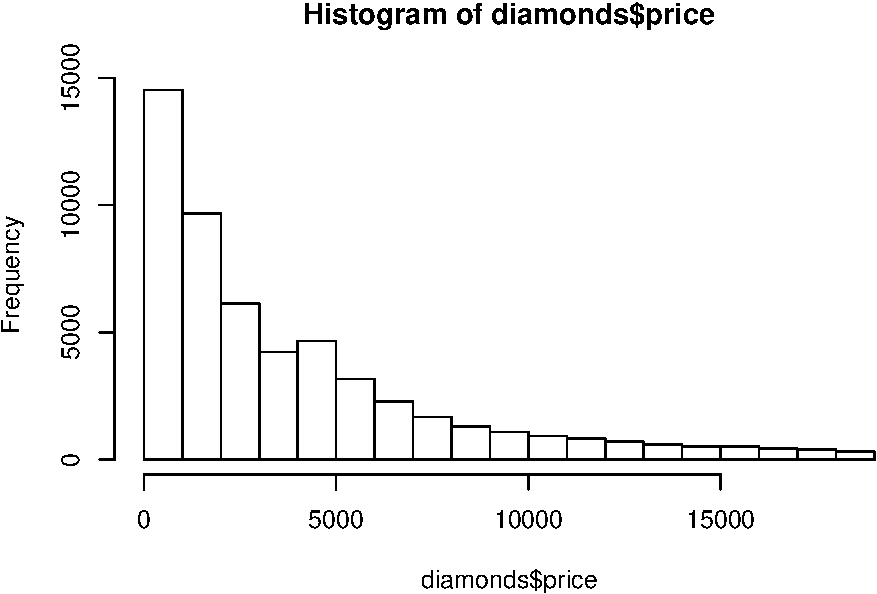
\includegraphics{_main_files/figure-latex/unnamed-chunk-47-1.pdf}

\begin{Shaded}
\begin{Highlighting}[]
\FunctionTok{boxplot}\NormalTok{(diamonds}\SpecialCharTok{$}\NormalTok{x)}
\end{Highlighting}
\end{Shaded}

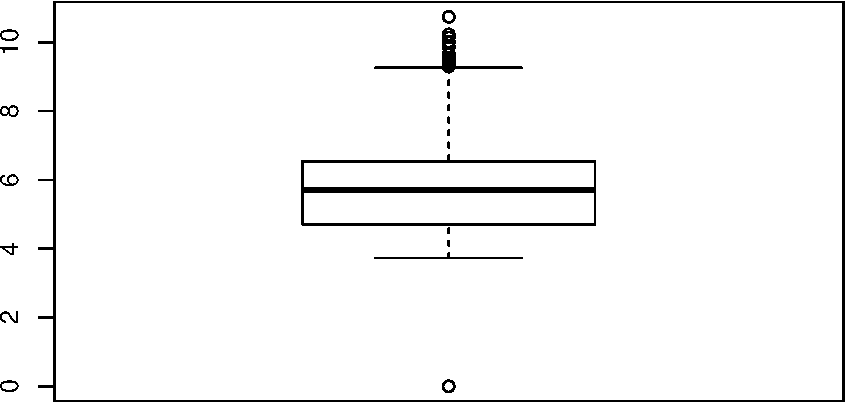
\includegraphics{_main_files/figure-latex/unnamed-chunk-48-1.pdf}

\hypertarget{visualisierung-mit-ggplot}{%
\subsection{\texorpdfstring{Visualisierung mit \texttt{ggplot()}}{Visualisierung mit ggplot()}}\label{visualisierung-mit-ggplot}}

Das Paket \texttt{ggplot2} ist Teil vom \texttt{tidyverse}. Hiermit lassen sich sehr flexible Graphiken gestalten. Wir werden ausschließlich mit diesem System arbeiten.

Die Syntax ist dabei auf den ersten Blick etwas komplexer.

Am Anfang steht der Befehl \texttt{ggplot(x)} mit dem Datensatz als Parameter

\begin{Shaded}
\begin{Highlighting}[]
\FunctionTok{ggplot}\NormalTok{(}\AttributeTok{data=}\NormalTok{diamonds)}
\end{Highlighting}
\end{Shaded}


\includegraphics{_main_files/figure-latex/unnamed-chunk-49-1.pdf}

Mit einem Mapping-Parameter legen wir die Dimensionen fest:

\begin{Shaded}
\begin{Highlighting}[]
\FunctionTok{ggplot}\NormalTok{(}\AttributeTok{data=}\NormalTok{diamonds, }\AttributeTok{mapping=}\FunctionTok{aes}\NormalTok{(}\AttributeTok{x=}\NormalTok{price, }\AttributeTok{y=}\NormalTok{carat))}
\end{Highlighting}
\end{Shaded}

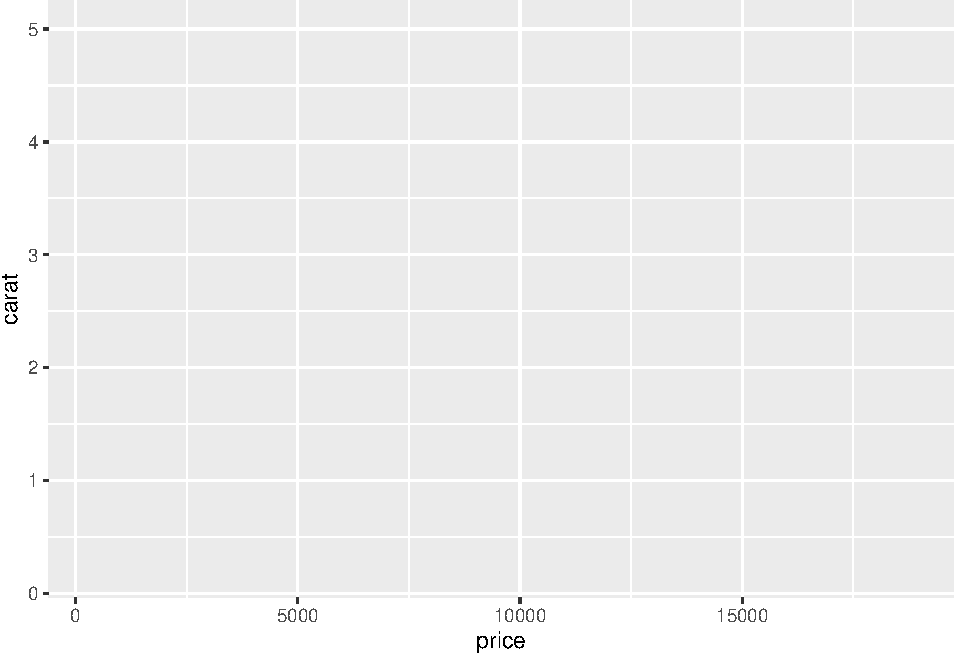
\includegraphics{_main_files/figure-latex/unnamed-chunk-50-1.pdf}

Das gleiche ohne Parameternamen:

\begin{Shaded}
\begin{Highlighting}[]
\FunctionTok{ggplot}\NormalTok{(diamonds, }\FunctionTok{aes}\NormalTok{(price, carat))}
\end{Highlighting}
\end{Shaded}

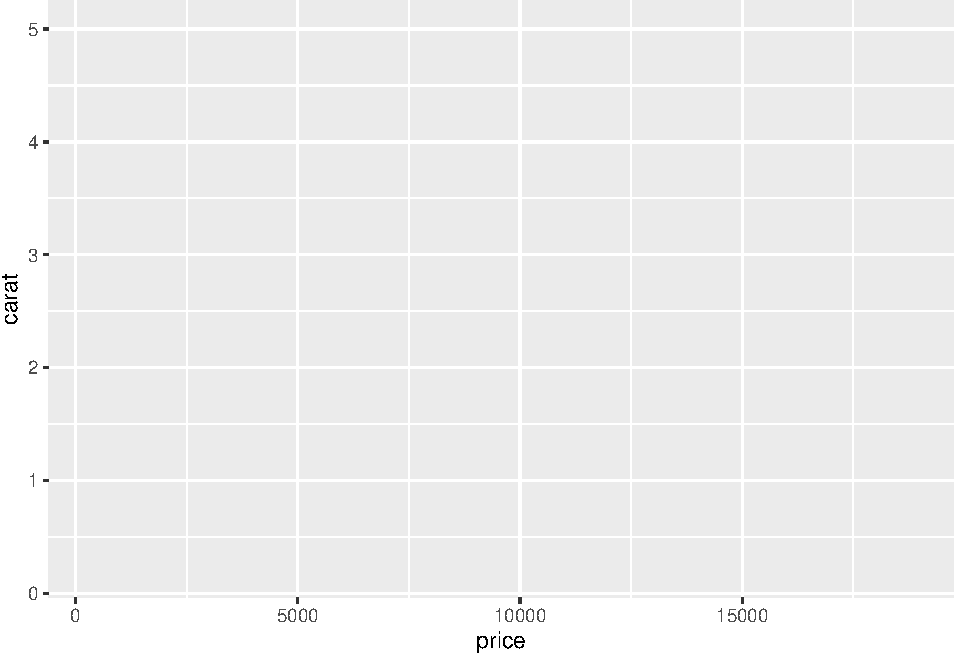
\includegraphics{_main_files/figure-latex/unnamed-chunk-51-1.pdf}

Nun kann mit dem \texttt{+}-Operator ein ``geometrischer'' Layer hinzugefügt werden:

\begin{Shaded}
\begin{Highlighting}[]
\FunctionTok{ggplot}\NormalTok{(diamonds, }\FunctionTok{aes}\NormalTok{(}\AttributeTok{x=}\NormalTok{carat, }\AttributeTok{y=}\NormalTok{price)) }\SpecialCharTok{+}
  \FunctionTok{geom\_point}\NormalTok{()}
\end{Highlighting}
\end{Shaded}

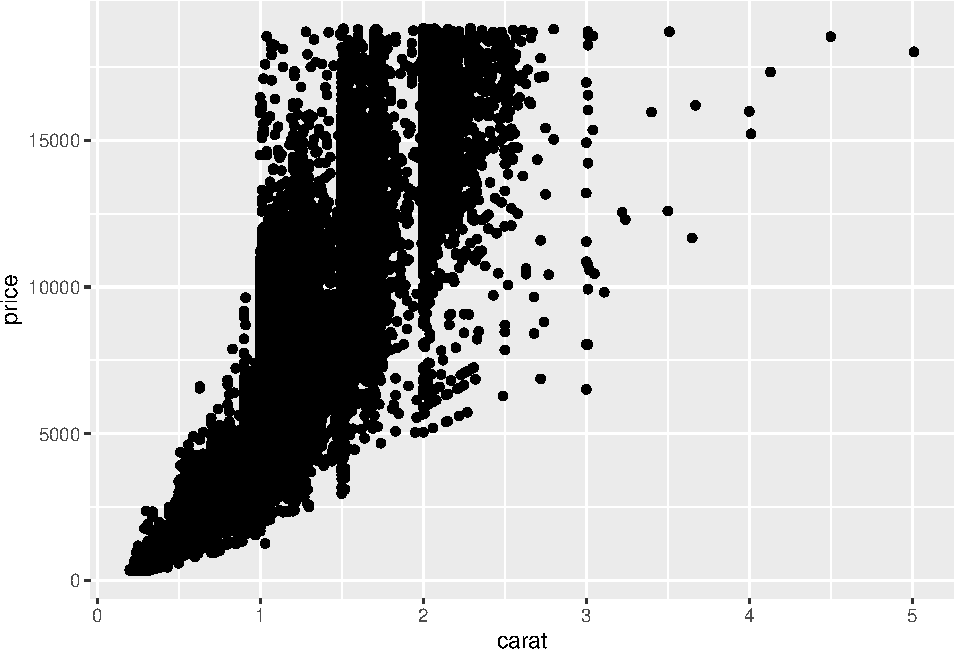
\includegraphics{_main_files/figure-latex/unnamed-chunk-52-1.pdf}

Weitere \texttt{geom}-Layer lassen sich mit dem \texttt{+}-Operator hinzufügen:

\begin{Shaded}
\begin{Highlighting}[]
\FunctionTok{ggplot}\NormalTok{(diamonds, }\FunctionTok{aes}\NormalTok{(}\AttributeTok{x=}\NormalTok{carat, }\AttributeTok{y=}\NormalTok{price)) }\SpecialCharTok{+}
  \FunctionTok{geom\_point}\NormalTok{() }\SpecialCharTok{+}
  \FunctionTok{geom\_smooth}\NormalTok{()}
\end{Highlighting}
\end{Shaded}

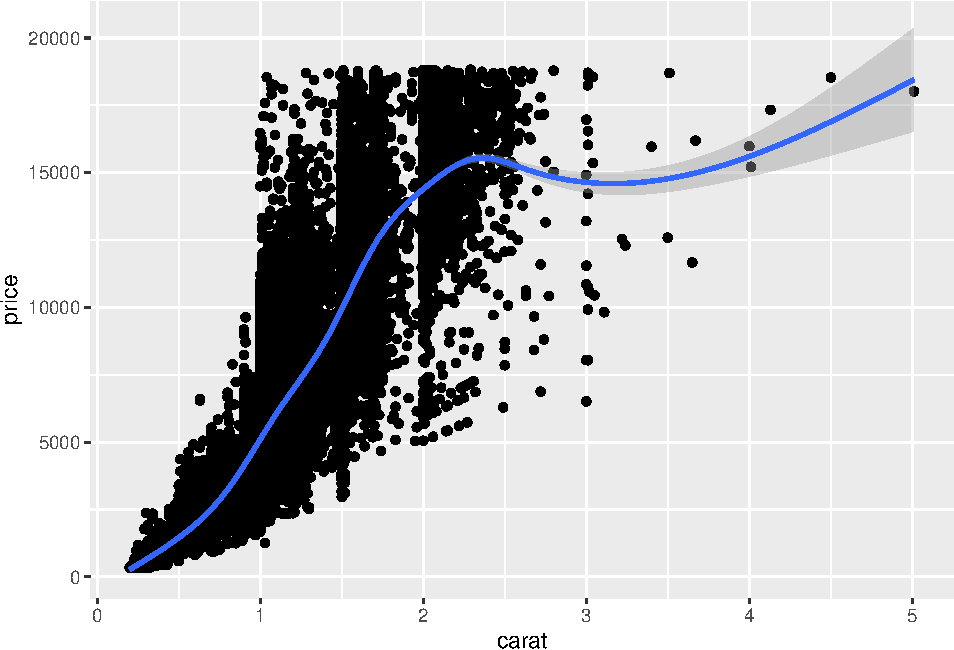
\includegraphics{_main_files/figure-latex/unnamed-chunk-53-1.pdf}

Die Layer-Funktionen können durch Parameter angepasst werden:

\begin{Shaded}
\begin{Highlighting}[]
\FunctionTok{ggplot}\NormalTok{(diamonds, }\FunctionTok{aes}\NormalTok{(}\AttributeTok{x=}\NormalTok{carat, }\AttributeTok{y=}\NormalTok{price)) }\SpecialCharTok{+}
  \FunctionTok{geom\_point}\NormalTok{(}\AttributeTok{size=}\FloatTok{0.5}\NormalTok{) }\SpecialCharTok{+}
  \FunctionTok{geom\_smooth}\NormalTok{(}\AttributeTok{color=}\StringTok{"red"}\NormalTok{)}
\end{Highlighting}
\end{Shaded}

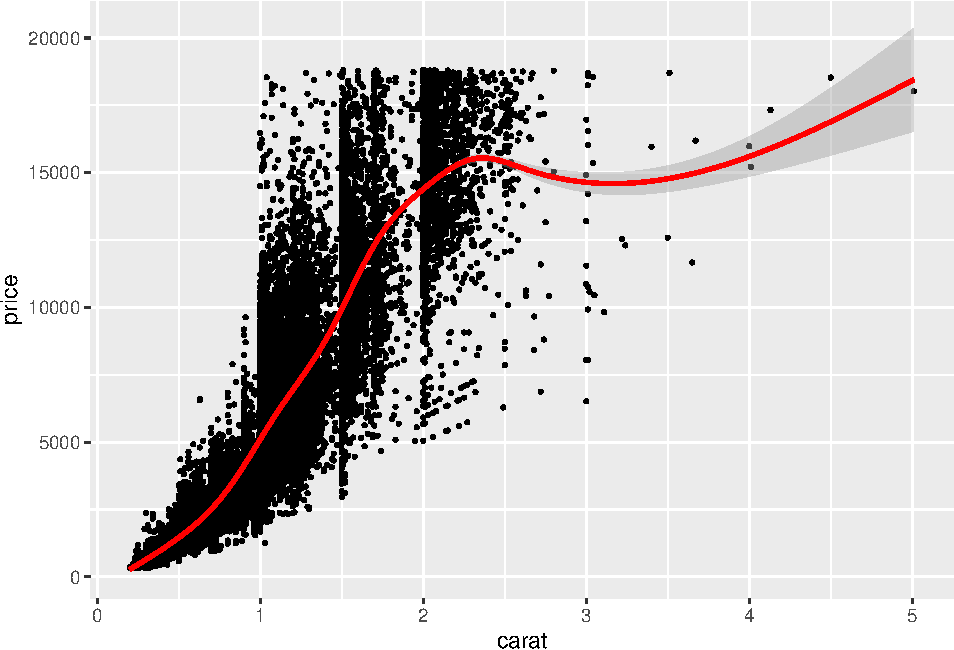
\includegraphics{_main_files/figure-latex/unnamed-chunk-54-1.pdf}

Dabei lassen sich in den einzelnen Layers mappings hinzufügen oder verändern:

\begin{Shaded}
\begin{Highlighting}[]
\FunctionTok{ggplot}\NormalTok{(diamonds, }\FunctionTok{aes}\NormalTok{(}\AttributeTok{x=}\NormalTok{carat, }\AttributeTok{y=}\NormalTok{price)) }\SpecialCharTok{+}
  \FunctionTok{geom\_point}\NormalTok{(}\FunctionTok{aes}\NormalTok{(}\AttributeTok{color=}\NormalTok{clarity), }\AttributeTok{size=}\FloatTok{0.5}\NormalTok{) }\SpecialCharTok{+}
  \FunctionTok{geom\_smooth}\NormalTok{(}\AttributeTok{color=}\StringTok{"red"}\NormalTok{)}
\end{Highlighting}
\end{Shaded}

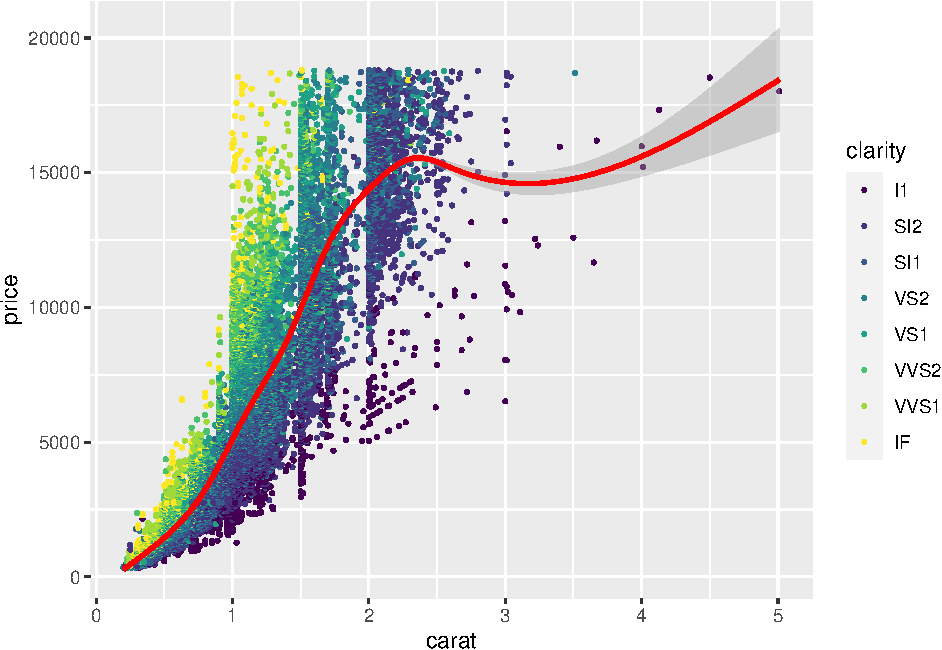
\includegraphics{_main_files/figure-latex/unnamed-chunk-55-1.pdf}

Schließlich lassen sich noch viele weitere optische Aspekte anpassen, z.B. Achsen, Farben, etc.:

\begin{Shaded}
\begin{Highlighting}[]
\FunctionTok{ggplot}\NormalTok{(diamonds, }\FunctionTok{aes}\NormalTok{(}\AttributeTok{x=}\NormalTok{carat, }\AttributeTok{y=}\NormalTok{price)) }\SpecialCharTok{+}
  \FunctionTok{geom\_point}\NormalTok{(}\FunctionTok{aes}\NormalTok{(}\AttributeTok{color=}\NormalTok{clarity), }\AttributeTok{size=}\FloatTok{0.5}\NormalTok{) }\SpecialCharTok{+}
  \FunctionTok{geom\_smooth}\NormalTok{(}\AttributeTok{color=}\StringTok{"red"}\NormalTok{) }\SpecialCharTok{+}
  \FunctionTok{scale\_x\_continuous}\NormalTok{(}\StringTok{"Karatzahl"}\NormalTok{, }\AttributeTok{breaks=}\FunctionTok{seq}\NormalTok{(}\DecValTok{0}\NormalTok{,}\DecValTok{5}\NormalTok{,}\FloatTok{0.5}\NormalTok{)) }\SpecialCharTok{+}
  \FunctionTok{scale\_y\_continuous}\NormalTok{(}\StringTok{"Preis"}\NormalTok{) }\SpecialCharTok{+}
  \FunctionTok{scale\_color\_brewer}\NormalTok{(}\StringTok{"Klarheit"}\NormalTok{) }\SpecialCharTok{+}
  \FunctionTok{theme\_dark}\NormalTok{()}
\end{Highlighting}
\end{Shaded}

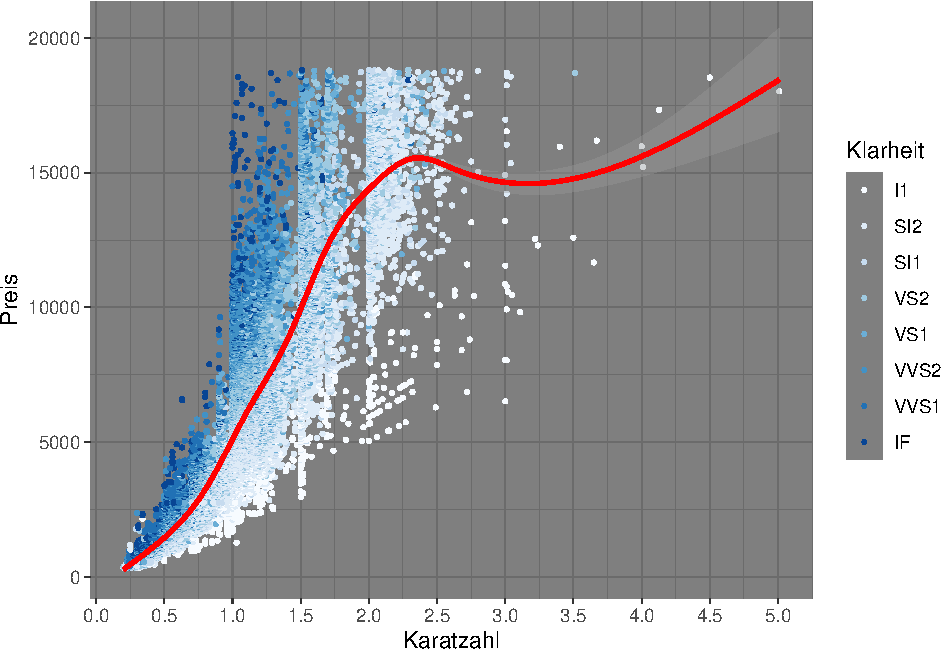
\includegraphics{_main_files/figure-latex/unnamed-chunk-56-1.pdf}

\hypertarget{aufgaben-2}{%
\subsection{Aufgaben}\label{aufgaben-2}}

Versuchen Sie, folgende Visualisierungen des Datensatzes \texttt{diamonds} auszugeben:

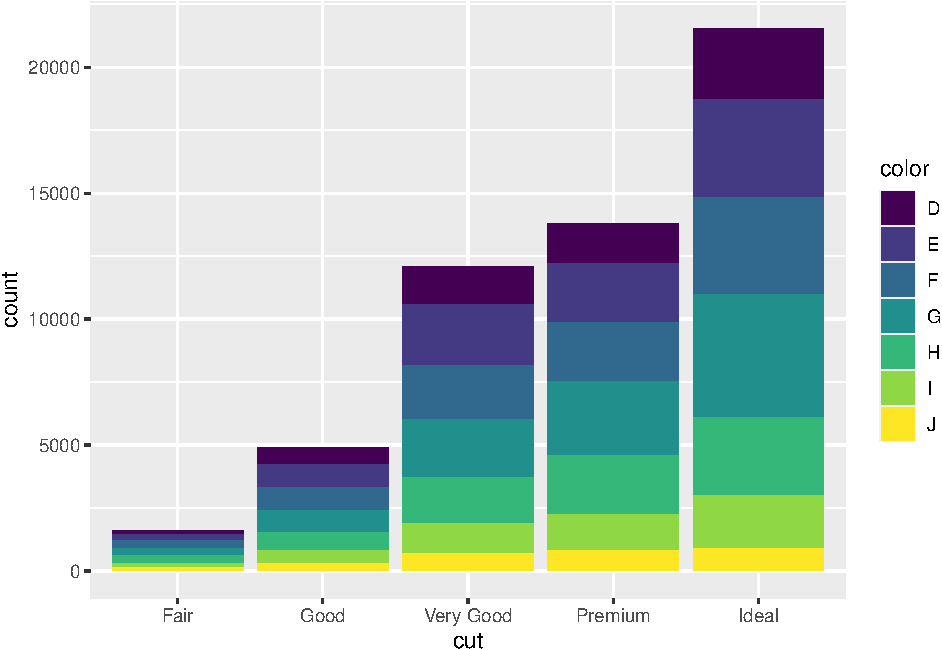
\includegraphics{_main_files/figure-latex/unnamed-chunk-57-1.pdf}

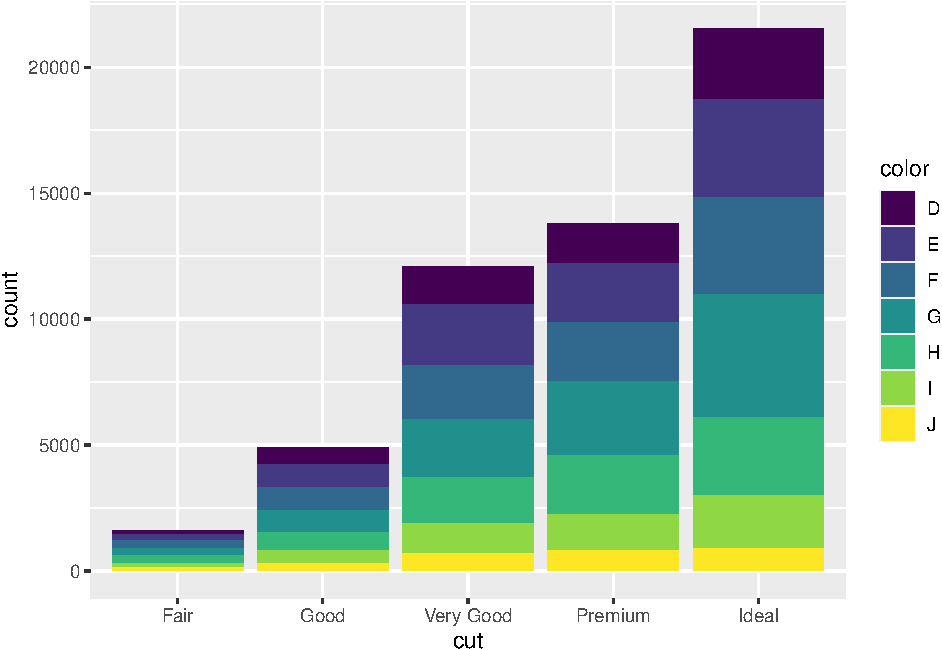
\includegraphics{_main_files/figure-latex/unnamed-chunk-58-1.pdf}

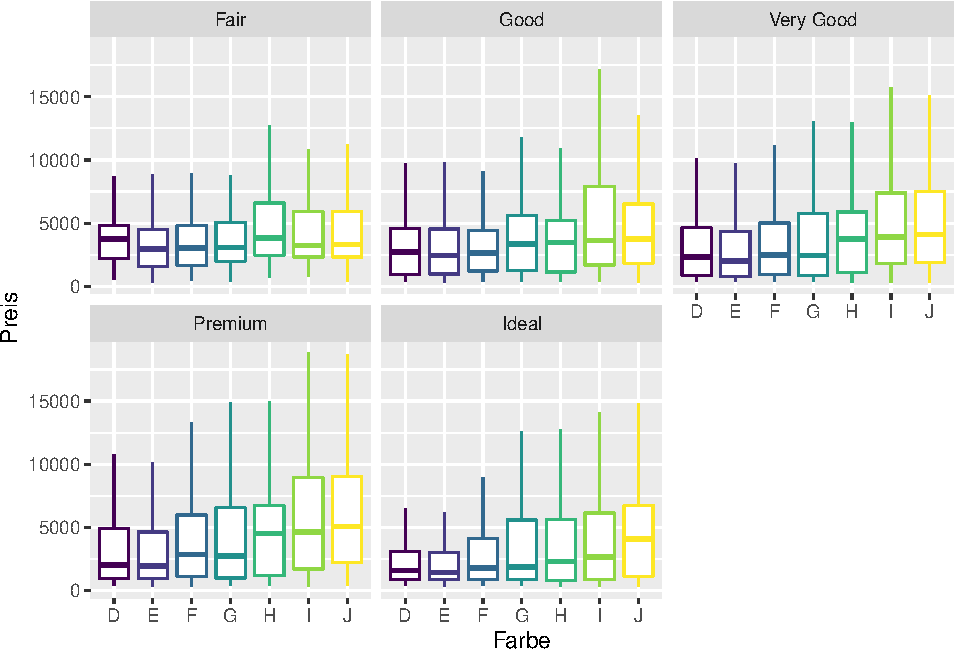
\includegraphics{_main_files/figure-latex/unnamed-chunk-59-1.pdf}

\hypertarget{r-for-data-science}{%
\subsubsection{R for Data Science}\label{r-for-data-science}}

Schauen Sie sich die Publikation \href{https://r4ds.had.co.nz/}{R for Data Science} an.

Was ist das für ein Buch? Wer ist das Zielpublikum?

Lesen Sie das Kapitel ``3: Data Visualization'' und vollziehen Sie die Visualisierungen nach.

Bearbeiten Sie die Aufgaben.

Bearbeiten Sie die \href{https://rstudio.cloud/learn/primers/3}{RStudio Primers zu Datenvisualisierung}.


\end{document}
